\documentclass[twoside,11pt]{article}
\usepackage{jair,theapa, rawfonts}

% Use the postscript times font!
\usepackage{times}

%my stuff
\usepackage{amssymb}
\usepackage{amsthm}
\usepackage{amsmath}
\usepackage{algorithm}
\usepackage[noend]{algpseudocode}
\usepackage{float}
\usepackage[titletoc,toc,title]{appendix}
\usepackage{fixltx2e}
\usepackage{dblfloatfix}
\usepackage{subcaption}
\usepackage{multirow}
\usepackage{ctable}


%mby

%\usepackage[authoryear]{natbib}
\usepackage{graphicx}

\raggedbottom %nicer enumerate
\theoremstyle{definition}
\newtheorem{defn}{Definition}[section]

%\jairheading{1}{2015}{3-17}{6/91}{9/91}
%\ShortHeadings{Recursive Feature Generation for Knowledge-based Induction}
%{Friedman \& Markovitch}
%\firstpageno{25}

%\title{Recursive Feature Generation for Knowledge-based Induction}
%\author{\name Lior Friedman \email liorf@cs.technion.ac.il \\
%	\name Shaul Markovitch \email shaulm@cs.technion.ac.il \\
%	\addr Technion-Israel Institute of Technology\\
%	Haifa 32000, Israel
%}

\begin{document}
	
%\maketitle

\thispagestyle{empty}

\begin{center}
{\LARGE Recursive Feature Generation\\ for Knowledge-based Induction}\\[0.2\baselineskip]
\end{center}

\begin{center}
{\large Research Thesis
In Partial Fulfilment of The Requirements for the Degree of
 \\Master of Science in Computer Science}
\end{center}

\vspace*{2\baselineskip}

\begin{center}
{\Large Lior Friedman}
\end{center}

\vspace*{8\baselineskip}


\begin{center}
Submitted to the Senate of the Technion - Israel Institute of Technology\\
Adar, 5777, Haifa, May, 2017
\end{center}

\clearpage
\thispagestyle{empty}

\tableofcontents

\clearpage
\thispagestyle{empty}

\listoffigures

\thispagestyle{empty}

\listoftables
\clearpage

\thispagestyle{empty}


\begin{abstract}
	When humans perform inductive learning, they often enhance the process by using extensive background knowledge.
	 Recently, a large collection of common-sense and domain specific relational knowledge bases have become available on the web.
	With the increasing availability of well-formed collaborative knowledge bases, it is possible to significantly enhance the performance and accuracy of existing learning by finding a way to effectively exploit these knowledge bases. 
	In this work, we present a novel supervised algorithm for injecting external knowledge into induction algorithms using a feature generation framework. Given a feature, the algorithm defines a new learning task over its set of values, and uses the knowledge base to solve the constructed learning task. The resulting classifier is then used as a new feature for the original problem.
	This approach allows us to make use of existing methods in machine learning to better generate our features.
	We have applied our algorithm to the domain of text classification using large semantic knowledge bases such as YAGO2 and Freebase. We have shown that the generated features significantly improve the performance of existing learning algorithms.
	Additionally, we have shown that our approach performs significantly better than another, unsupervised feature generation method, thus demonstrating the unique benefits of our approach.
\end{abstract}

\clearpage
\pagenumbering{arabic}


\section{Introduction}
\label{sec:Intro}
In recent decades, machine learning techniques have become more prevalent in a wide variety of fields. %such as medical diagnosis, vision, and biology.
Most of these methods rely on the inductive approach: given a set of labeled examples, they attempt to locate a hypothesis that is heavily supported by the known data. These methods have proven themselves successful when the number of examples is sufficient, and a collection of good,
distinguishing features is available.
In many real-world applications, however, the given set of features is not sufficient for inducing a high quality classifier.

One approach for overcoming this difficulty is to generate new features that are combinations of the given ones.
For example, the LFC algorithm \shortcite{ragavan1993complex} combines binary features through the use of logical operators such as $\land ,\lnot$.
Another example is the LDMT algorithm \cite{utgo1991linear}, which generates linear combinations of existing features.
Deep Learning methods combine basic and generated features using various activation functions such as sigmoid or softmax.
The FICUS framework \cite{markovitch2002feature} presents a general method for generating features using any given set of constructor functions.

The above approaches are limited in that they merely combine existing features to make the representation more suitable for the 
learning algorithm.   While this approach often suffices, there are many cases where additional information is required for successful classification.
When people perform inductive learning, they usually rely on a vast body of background knowledge to make the process more
effective \cite{mcnamara1996learning}. For example, assume two positive examples of people suffering from some genetic disorder, where the 
value of the country-of-origin feature is Poland and Romania.  Existing induction algorithms, including those generating features 
by combination, will not be able to generalize over these two examples.  Humans, on the other hand, can easily generalize 
and generate a new feature, \emph{Eastern Europe}, based
on their general background knowledge.

In this work, we present a novel algorithm that uses a similar approach for enhancing inductive learning with background knowledge through feature generation.
Our method assumes a given body of knowledge represented in relational form.  The algorithm treats feature values as objects and constructs new learning problems, using the background relational knowledge as their features.  The resulting classifiers are then used as new generated features.
For example, in the above very simple example, our algorithm would have used the \emph{continent} and \emph{region} features of a country,
inferred from a geographic knowledge base, to create the new feature that makes generalization possible.  Using background knowledge in the form of generated features allows us to utilize existing powerful learning algorithms for the induction process.

We implemented our algorithm in the domain of text classification problems, using Freebase and YAGO2 as our background knowledge bases, 
and performed an extensive set of experiments to test the effectiveness of our method.  Results show that the use of background knowledge significantly improves the classification accuracy of existing learning algorithms.

\section{Motivation} \label{motivation}

Before we delve into the detailed description of our algorithm, we would like to illustrate its main ideas using an example.
Suppose we are attempting to identify people with a high risk of suffering from a genetic disorder. Assume that the target concept to be discovered is that those at risk are women with ancestors originating from desert areas. To identify patients at risk, we are given a training sample of sick and healthy people, containing various features, including gender and their full name. We call this learning problem $T_1$.
Assuming we have no additional information, an induction algorithm (a decision tree learner, in this example) would likely produce a result similar to that shown in Figure \ref{fig:tree_base}. While such a classifier will achieve a low training error, the hundreds of seemingly unrelated surnames will cause it to generalize poorly. %This phenomenon is known as over-fitting, meaning the model is too adjusted to known data and cannot generalize to previously unseen examples. We can intuitively see this in Figure \ref{fig:tree_base}, as each leaf hypothesis is supported by only a single example.

\begin{figure}[h]
	\centering
	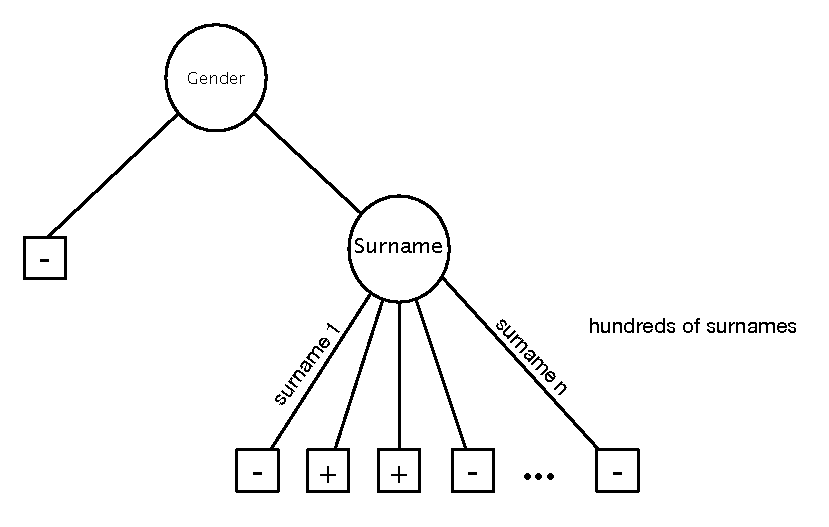
\includegraphics[width=0.8\linewidth]{fig1.pdf}
	\caption{A decision tree for the basic features}
	\label{fig:tree_base}
\end{figure}

The above example illustrates a case where, without additional knowledge, an induction algorithm will yield a very poor result. %Even if we attempt to use standard feature generation approaches, there is no additional information that combinations of these features would find.
However, if we assume access to a relational knowledge base connecting surnames to common countries of origin, we can begin to apply our knowledge-based feature generation techniques to the problem, as we can move from the domain of surnames to that of countries. 
Our algorithm does so by creating a new learning problem, $T_2$. The training objects for learning problem $T_2$ are surnames; surnames of people at risk are labeled as positive. The features for these new objects are extracted from the knowledge base. In this case, we have a single feature: the country of origin.
Solving the above learning problem through an induction algorithm yields a classifier on surnames that distinguishes between surnames of people at risk and surnames of healthy individuals. This classifier for $T_2$ can then be used as a binary feature for the original problem $T_1$ by applying it to the feature value of surname. For example, it can be used as a feature in the node corresponding to people whose gender is female in Figure \ref{fig:tree_base}, yielding the tree seen in Figure \ref{fig:lvl1_tree}. 

This new feature gives us a better generalization over the baseline solution, as we now abstract the long list of surnames to a short list of countries. %We can see this as nodes in the classifier for $T_2$ are derived from multiple surnames. 
This result also allows us to capture previously unseen surnames from those countries. However, this is not a sufficient solution, as we have no way of generalizing on previously unseen countries of origin. %, and some countries may not have sufficient representation to induce an accurate classifier. %talk about not concept?


\begin{figure}[h]
	\centering
	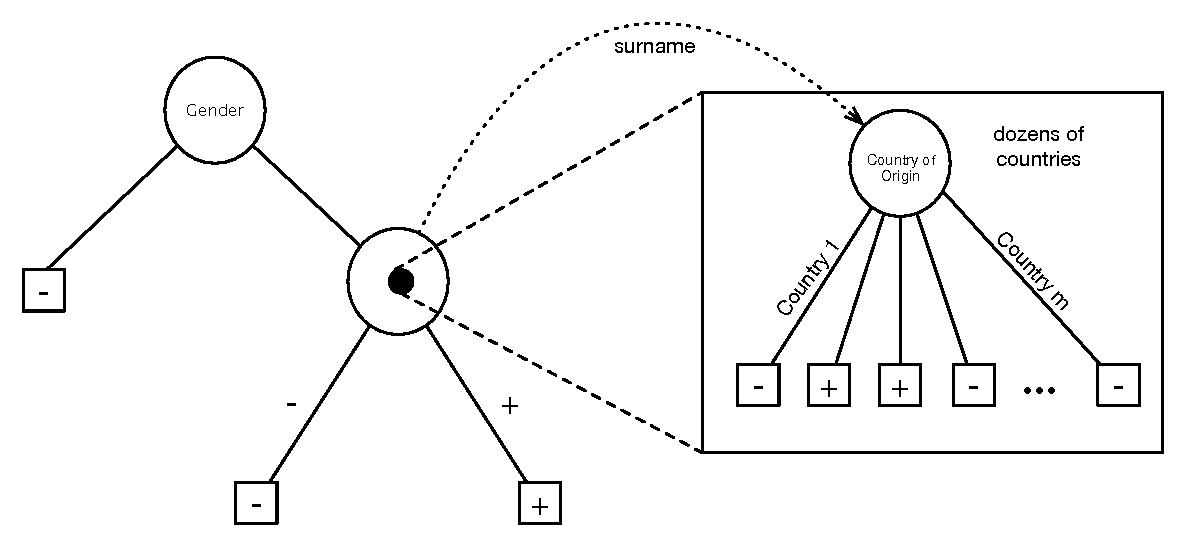
\includegraphics[width=\linewidth]{fig2.pdf}
	\caption{A constructed feature used within a decision tree}
	\label{fig:lvl1_tree}
\end{figure}

If, however, we would have recursively applied our method for solving $T_2$, we could have obtained a better generalization.
When learning to classify surnames, our method creates a new learning problem, $T_3$, with countries as its objects. Countries of surnames belonging to people with high risk are labeled as positive. The knowledge base regarding countries is then used to extract features for this new training set.
Applying a standard learning algorithm to $T_3$ will yield a classifier that distinguishes between countries of origin of people at risk and those not at risk by looking at the properties of countries and concluding that countries with high average temperature and low precipitation, the characteristics of desert areas,  are indicative of high risk. 

\begin{figure*}[th]
	\centering
	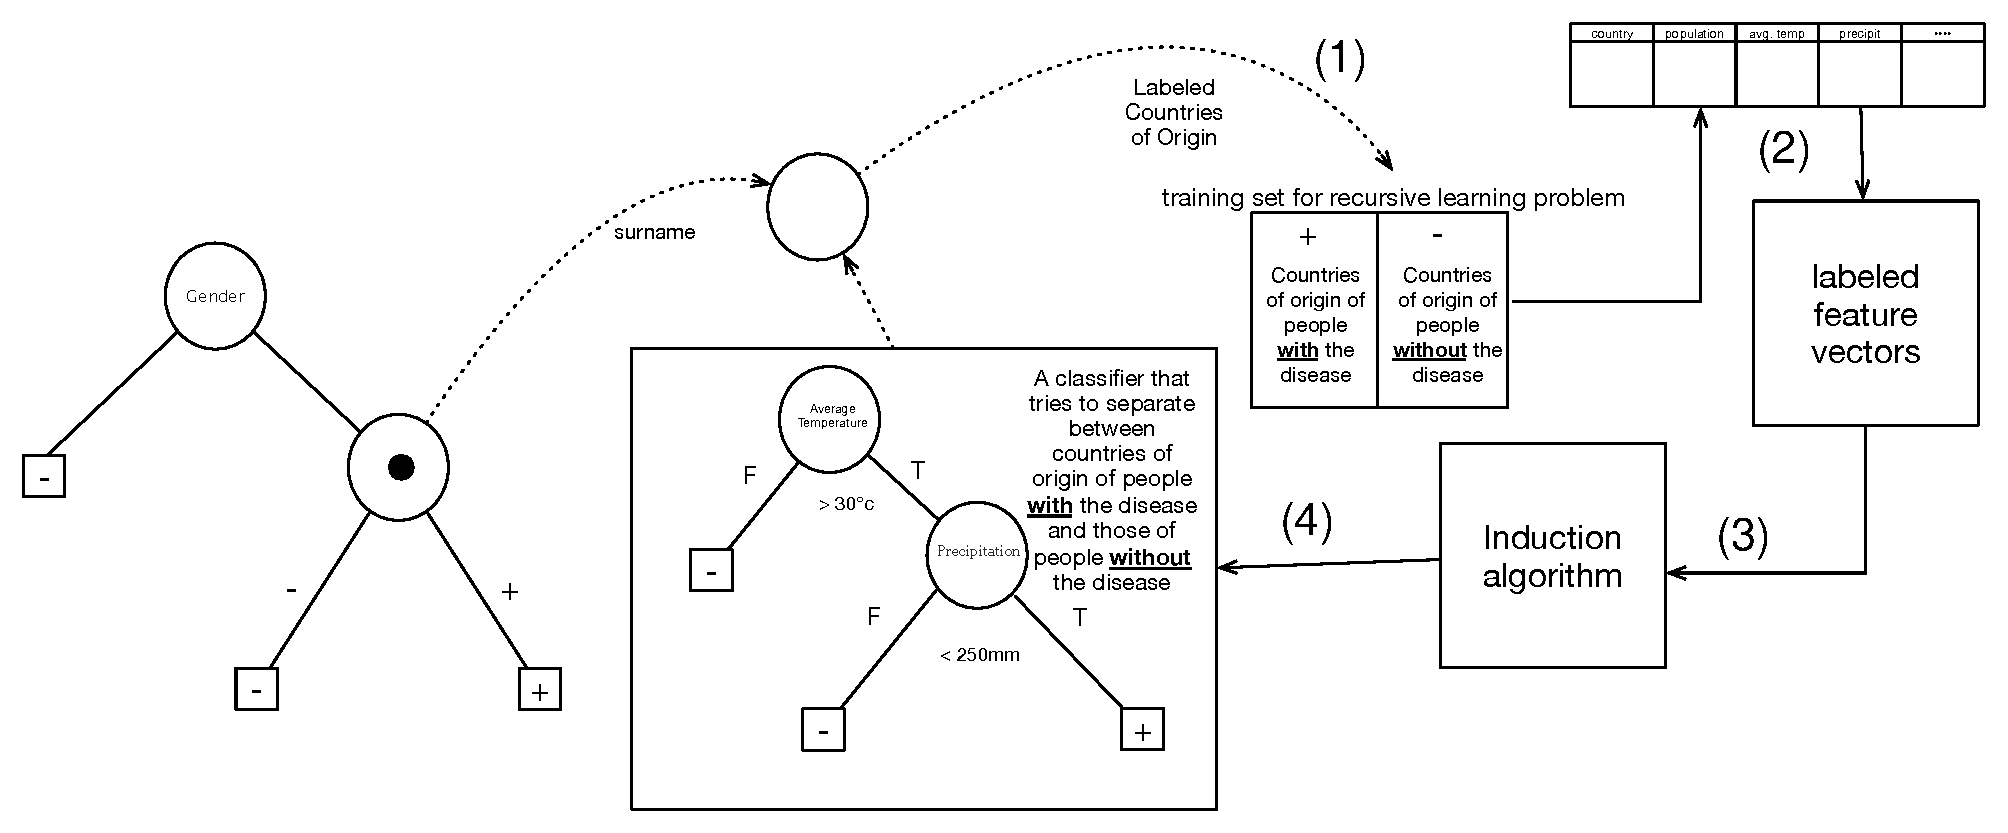
\includegraphics[width=0.9\linewidth,height=0.33\linewidth]{fig4_annotated.pdf}
	\caption{Recursive construction of a learning problem on countries of origin. $(1)$ Creating the objects for the new problem. $(2)$ Creating features using the knowledge base. $(3)$ Applying an induction algorithm. $(4)$ The resulting feature.}
	\label{fig:moving_to_lvl2}
\end{figure*}

The result of this process, depicted in Figure \ref{fig:moving_to_lvl2}, is a new feature for $T_2$, that is, a feature on surnames. This feature is then used to construct a classifier for $T_2$, which is used in turn as a feature for $T_1$, yielding a feature on people. This new feature for people, shown in Figure \ref{fig:lvl2_tree}, will check whether their surname corresponds to a country of origin that has desert-like characteristics. 
%TODO:this part
This example illustrates the major steps of our approach: the construction of new induction problems on feature values using the given knowledge base, the creation of classifiers over the above learning problems, and the use of said classifiers as new features. These steps allow us to accurately capture the target concept using a two-level recursive process.

\begin{figure*}[th]
	\centering
	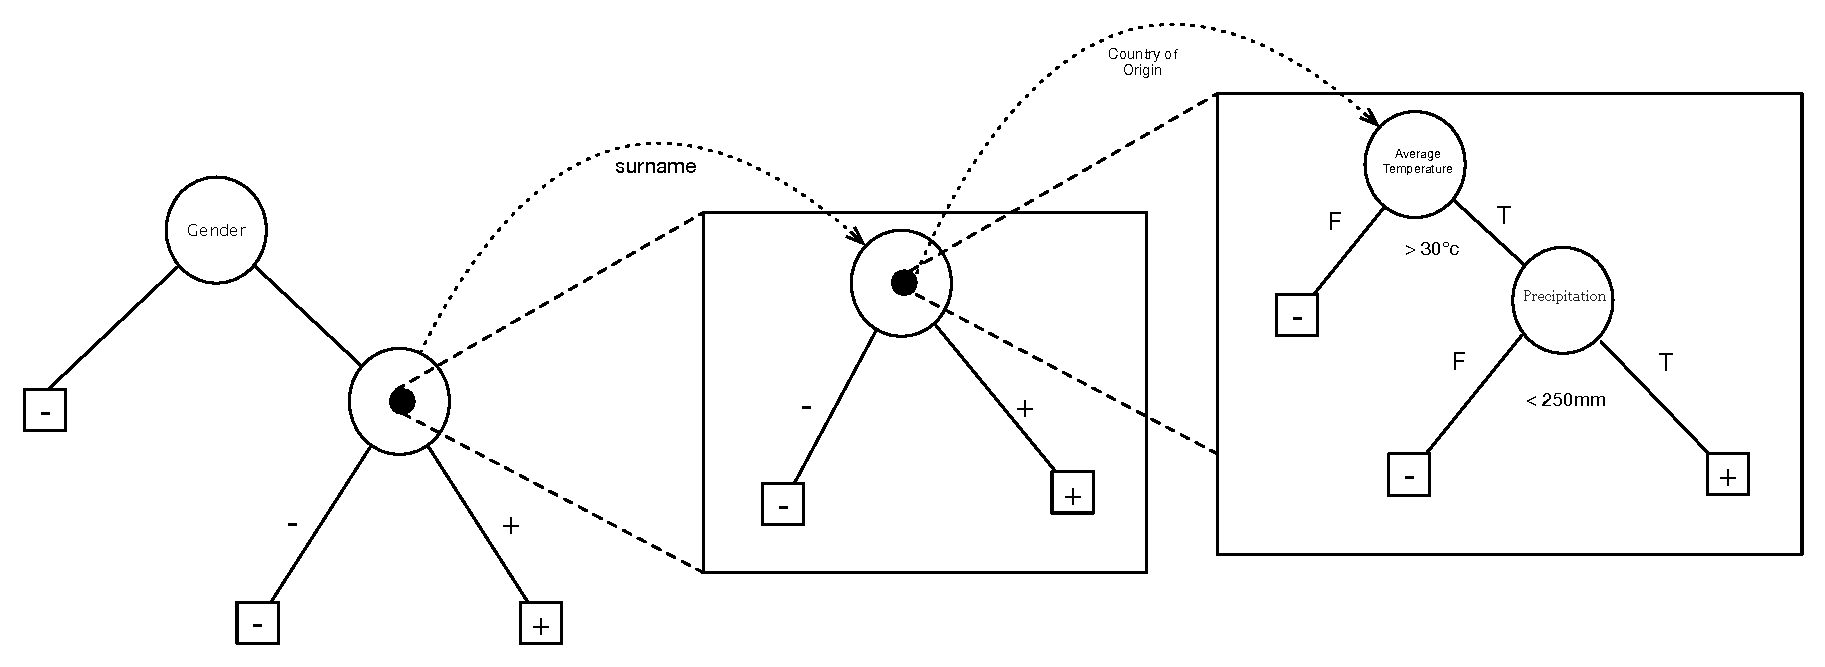
\includegraphics[width=\linewidth]{fig3.pdf}
	\caption{A two-level constructed feature used within a decision tree}
	\label{fig:lvl2_tree}
\end{figure*}



%%%%%%%%%%%%%%%%%%%%%%%%%%%%%%%%%%%%%%%%%%%%%%%%%%%%%%%%%%
\section{Generating Features through Recursive Induction} \label{formal}
%%%%%%%%%%%%%%%%%%%%%%%%%%%%%%%%%%%%%%%%%%%%%%%%%%%%%%%%%%

In the following sections, we formally define the feature generation problem, present a solution  in the form of a simple algorithm that generates features by using
relational expansions, and then proceed to describe our main recursive feature generation algorithm.

\subsection{Problem Definition}

We begin our discussion with a standard definition of an induction problem. 
Let $O$ be a set of objects. Let $Y=\{0,1\}$ be a set of labels\footnote{We assume binary labels for ease of discussion.}. Let $C:O\rightarrow Y$ be a target concept. Let $S=\{(o_{1},y_{1}),\ldots,(o_{m},y_{m})\}$ be a set of labeled examples such that $o_{i}\in O, y_{i}\in Y, C(o_i)=y_i$. 
Let $F=\{f_{1},\ldots,f_{n}\}$ be a \emph{feature map}, a set consisting of several \emph{feature functions} $f_{i}:O\rightarrow I_{i}$.  This definition implies a training set represented by feature vectors: $S_F=\{ (\langle f_1(o_i),\ldots,f_n(o_i)\rangle, y_i) | (o_i,y_i) \in S\}$. A learning algorithm $L$ takes $S_F$ as inputs, and outputs a classifier $h_{S_F}:O\rightarrow Y$.
\begin{defn}
	Let $L(S,F)=h_{S_F}$ be the classifier given as an output by $L$ given $\langle S,F\rangle$. Assuming $S\sim D$, the generalization error of a learning algorithm $L$ is the probability $Pr(h_{S_F}(x)\neq y)$, where $(x,y)\sim D$.
\end{defn}

\begin{defn}
	A \emph{feature generation algorithm} $A$ is an algorithm that, given $\langle S,F\rangle$, creates a new feature map $F'=\{f'_{1},\ldots,f'_{l}\}, f'_{k}:O\rightarrow I_k$.
\end{defn}

In order to evaluate the output of a feature generation algorithm $A$, we must define its utility. Given $\langle S,F \rangle$, $A$ generates a feature set $F'_A$.
Given $S\sim D$, a feature set $F$, a generated feature set $F'_A$ and a learning algorithm $L$, the utility of $A$ is $U(A(S,F))=Pr(h_{S_F}(x)\neq y)-Pr(h_{S_{F'_A}}(x)\neq y)$, where $(x,y)\sim D$.

Thus, in order for the utility of $A$ to be positive, the generated feature set $F'_A$ must yield a lower generalization error than the original feature map $F$.

In this work, we assume that, in addition to $S_F$, $A$ also has access to a set of binary\footnote{If our relations are not binary, we can use projection to create multiple binary relations instead.} relations ${\cal R}=\{R_{1},\ldots,R_{t}\}, R_j:D_j\times D_{j'}$ representing our knowledge base. 
\begin{defn}
	A \emph{knowledge-based feature-generation algorithm} $A$ is an algorithm that, given $\langle S,F,{\cal R} \rangle$, creates a new feature map $F_{{\cal R}}=\{f'_{1},\ldots,f'_{l}\}, f'_{k}:O\rightarrow I_k$.
\end{defn}

%TODO: this
By using a feature generation algorithm based on a set of relations ${\cal R}$, we would like to achieve a higher utility than that achieved without ${\cal R}$. We assume that some feature values are also relation keys, allowing us to apply these relations to our learning problem. More formally, we assume that
$\bigcup_{f_i} I_i \cap \bigcup_{R_j} D_j \neq \emptyset$. 

\subsection{Expansion-Based Feature Generation} \label{shallow_section}

Our first method for knowledge-based feature generation ignores the labels of the original learning problem.
The algorithm extends each feature value by all of the tuples it appears in.
Let $f_i$ be an original feature. Let $R_j:D_j\times D_{j'}$ be a relation such that  $Image(f_i) \subseteq D_j$. We can generate a new feature function $f_{i,j}:O\rightarrow D_{j'}$ by composing $R_j$ onto $f_i$, yielding our new feature function  $f_{i,j}(x)=R_j\circ f_i$. For example, if $f_i$ lists a person's country of origin, and $R_j$ maps countries to their continent, then $f_{i,j}$ lists a person's continent of origin.

%Another case that must be discussed is the case where some values of $f_i$ cannot be expanded as above, meaning $Image(f_i) \not\subset D_j$ but $Image(f_i) \cap D_j \neq\emptyset$. We can resolve this in a manner similar to missing features in induction problem, by treating $R_j$ as a partial function from $Image(f_i)$ to $D_{j'}$. In order to complete this partial function, we first mark \emph{undefined} as $\perp$. We can turn $R_j$ into a full function with regards to $Image(f_i)$ as follows: $\tilde{R}_j(x)=\begin{cases} R_j(x) &\mbox{if } x\in D_j\\ 
%\perp & \mbox{otherwise } \end{cases}$.
%The result is a full function $\tilde{R}_j:Image(f_i)\cup D_j\rightarrow D_{j'}\cup\{\perp\}$. We also note that the same process can be applied to cases where $R_j$ has missing values\footnote{This is usually the case in human curated knowledge bases.}, meaning it is a partial function with regards to $D_j$. 

In the general case, composing $R_j$ onto $F_i$ yields a set of values, meaning that $f_{i,j}(x)=\{v\in D_{j'}|(f_i(x),v)\in R_j\}$. 
To yield a single value, we use an aggregation function on this set.
An aggregation function is a function that, given a multi-set as input, outputs a single value. There are many types of aggregators, such as numerical aggregators (e.g. sum), categorical aggregators (e.g. most common member) and binary aggregation functions (e.g. exists).
For the experiments described in this paper, we use  
two aggregation function types: Majority and Any, but in general any other reasonable aggregation function can be used instead.
The Majority aggregator, for example, is defined as follows.  For each value $v\in D_{j'}$, we generate a binary feature function with value 1 only if $v$ is the majority value: 
$Majority^v(X)=1 \iff majority(X)=v$.
The pseudo-code of this algorithm (called   
\emph{Expander-FG}) is listed in Algorithm \ref{code-compete}.

%Now that we have considered the possible behaviours of a given relation $R_j$, we can proceed to define the \emph{Expander-FG} feature generation algorithm. Given a feature $f_i$, \emph{Expander-FG} will go over the relations within the knowledge base and attempt to create features $f_{i,j}:O\rightarrow D_{j'}\cup\{\perp\}$ through the discussed techniques. \emph{Expander-FG} then gathers all generated features and outputs them. The pseudo-code is given below.

\begin{algorithm}[H]
	\caption{\emph{Expander-FG}}
	\label{code-compete}
	\small
	$\sigma$ - An aggregation function family
	\begin{algorithmic}
		\Function{GenerateFeatures}{$S$,$F$, ${\cal R}$}
		\State $generated=\emptyset$
		\For {$f_i \in F$}
		\For {$R_j \in {\cal R}$ such that $Image(f_i)\subseteq D_{j}$ }
		\If {$R_j$ is a function}
		%\If {$Image(f_i)\subseteq D_{j}$}
		%\State add $\{f_{i,j}=R_j\circ f_i\}$ to $generated$
		\State add $\{f_{i,j}=R_j\circ f_i\}$ to $generated$
		\Else \Comment $R_j$ is a relation $R_j:D_j\times D_{j'}$
		\State add $F^\sigma_{i,j}=\{\sigma^v(f_{i,j})|v\in D_{j'}\}$ to $generated$
		\EndIf
		\EndFor
		\EndFor
		\State \Return $generated$ 
		\EndFunction
		
	\end{algorithmic}
\end{algorithm}

\subsection{Recursive Feature Generation Algorithm}
\label{algorithm_section}
One way to extend the \emph{Expander-FG} algorithm described in the previous section is to apply it repeatedly to its own output.
Extending the algorithm in this fashion, however, would yield an exponential increase in the number of generated features, making deep connections very difficult to discover.
We therefore propose an alternative knowledge-based feature generation algorithm. Given an input $\langle S,F,{\cal R} \rangle$, for each feature $f_i\in F, f_i:O\rightarrow I_i$, our algorithm creates a recursive learning problem whose objects are the values of $f_i$, where values associated with positive examples in $S$ are labeled positive. %, and those associated with negative examples labeled negative. 
Features for this generated problem are created using the relations in ${\cal R}$. Once this new learning problem $\langle S'_i,F_{\cal R}\rangle$ is defined, a learning algorithm is used to induce a classifier $h_i:I_i\rightarrow Y$. Finally, our algorithm outputs a single generated feature for $f_i$, $f'_i(x)=h_i\circ f_i=h_i(f_i(x)), f'_i:O\rightarrow Y$.
We note that during the induction process of the newly created learning problem, we can apply a feature generation algorithm on $\langle S'_i,F_{\cal R},{\cal R} \rangle$. In particular, we can apply the above method recursively to create additional features. We call this algorithm \emph{FEAGURE} (FEAture Generation Using REcursive induction).

%\subsubsection{Creating Learning Problems using Relations}  

Given a feature $f_{i}$, we create a recursive learning problem $\langle S'_i,F_{\cal R} \rangle$. %In this section, we will discuss how we do so.
Let $v_i(S) = \{v | (o,y) \in S, f_{i}(o)=v\}$ be the set of feature values for $f_i$ in the example set $S$. %In the intro example, for instance, $v_i(S)$ will be the set of all last names of patients that appeared in the training set.
We use $v_i(S)$ as our set of objects. To label each $v \in v_i(S)$, we first examine the labels in the original problem.
If there is a single example $o \in S$ such that $f_i(o)=v$, then the label of $v$ will be the label of $o$. Otherwise, we take the majority label of examples whose feature value is $v$. We can state this more formally as follows: if $s_i(v)=\{o | (o,y)\in S, f_{i}(o)=v\}$ is the set of objects whose feature value is $v$, then $label(v)=majority(\{y|(o,y)\in S, o\in s_i(v)\})$.

%We now formulate a new learning problem with the constructed training set
%$S'_i = \{ (v, label(v)) | v \in v_i(S) \}$.
To fully define our learning problem, we must specify a feature map over $v_i(S)$. In a similar manner to \emph{Expander-FG}, we use the relations in ${\cal R}$ on the elements in the new training set $S'_i = \{ (v, label(v)) | v \in v_i(S) \}$.
For each $R_j\in {\cal R}$, if it is relevant to the problem domain, meaning that $v_i(S)\subseteq D_j$, we utilize it as a feature by applying it to $v$. If $R_j(v)$ is a set, we use aggregators, as described in the previous section. 
The result of this process is a generated feature map for $S'_i$, denoted as $F_{\cal R}$. 

We now have a new induction problem $\langle S'_i,F_{\cal R} \rangle$.
We can further extend $F_{\cal R}$ by recursively using \emph{FEAGURE}, yielding a new feature map $F'_{\cal R}$. The depth of recursion is controlled by a parameter $d$, which is usually set according to available learning resources.
We proceed to use a learning algorithm\footnote{For the experiments described in this paper, we used a decision tree learner, but any induction algorithm can be used.} on $\langle S'_i,F'_{\cal R} \rangle$ in order to train a classifier, giving us $h_i:I_i\rightarrow Y$. We can then use $h_i$ on objects in $S$ as discussed above, yielding a new feature $f'_{i}(x)=h_{i}(f_{i}(x)), f'_{i}:O\rightarrow Y$. 

It is important to note that these new features might over-fit the generated problem, especially if it is small or imbalanced. There are several known ways to combat this issue. For our experiments, we decided to apply the following filters:
\begin{itemize}
	\item We do not call the learner in cases where the generated learning problem has too few examples.
	\item We do not call the learner on a generated training set if it is a single set problem.
	\item We filter out generated features that have an information gain of zero on the (original or generated) training set.
\end{itemize}  

We found these criteria sufficient for disqualifying very poor features without requiring a significant change in our approach.

%TODO:mby-two level features: we have a set...

%TODO
The full algorithm is listed in Algorithm \ref{code-creating-prob}.
We note that this feature generation approach creates features that can be used alongside any induction algorithm. Additionally, any induction algorithm can be used to learn $h_i$. Due to this generality, the extensive knowledge and literature available for induction methods applies in full. Furthermore, the recursive nature of \emph{FEAGURE} allows for a structured search of the knowledge base, with each new recursive problem modeling a projection of the problem space to the new domain. For example, in the motivating example, we began by learning a problem regarding people at risk, which we projected to a new domain of surnames. We then re-contextualized that problem to the domain of countries, for which we induced a good solution. We proceeded to use this solution to resolve the original learning task concisely and accurately.

\begin{algorithm}[H]
	\caption{FEAGURE algorithm}
	\label{code-creating-prob}
	\small
	%insert param stuff
	\begin{algorithmic}
		\Function{GenerateFeatures}{$F$, $S$, ${\cal R}$, $d$}
		\For {$f_i\in F$}
		\State $S'_i,F_{\cal R}$= \Call{CreateNewProblem}{$f_i$,$S$,${\cal R}$,$d$} %\Comment{We can apply our algorithm recursively here}
		\State $h_i$= \Call{InductionAlgorithm}{$S'_i,F_{\cal R}$} 
		%\If {\Call{Compare}{$h_i,F$}} \Comment Compare $h_i$ to $F$
		\State add $f'_i(x)=h_i\circ f_i$ to generated features (unless disqualified)
		%\EndIf
		\EndFor
		\State \Return generated features
		\EndFunction
		\State 
		\Function{CreateNewProblem}{$f_{i}$, $S$, ${\cal R}$, $d$}
		\State $v_i(S) = \{v | (o,y) \in S, f_{i}(o)=v\}$
		\State		$S'_i =  \{ (v, \mbox{majority-label}(s_i(v))) | v \in v_i(S),		 s_i(v)=\left \{o | (o,y)\in S, f_{i}(o)=v \right \}  \} $
		
		
		\State $F_{\cal R}=\{R_j(v)| R_j\in{\cal R}, v_i(S)\subseteq D_j\}$
		\If {$d>0$}
		\State $F_{\cal R}=F_{\cal R}\cup$\Call{GenerateFeatures}{$F_{\cal R}, S'_i,  {\cal R}$, $d-1$}
		\EndIf
		\State \Return $S'_i, F_{\cal R}$ 
		\EndFunction
		
	\end{algorithmic}
\end{algorithm}

\subsection{Finding Locally Improving Features} \label{tree_usage}

Some generated features may prove very useful for separating only a subset of the training data but may be difficult to identify in the context of the full training data. In the motivating example in Section \ref{motivation}, for instance, examples of male individuals (who are not at risk) are irrelevant to the target concept, and thus mask the usefulness of the candidates for feature generation.

In this subsection, we present an extension of our \emph{FEAGURE} algorithm that evaluates features in local contexts using the divide \& conquer approach.
This algorithm uses a decision tree induction method as the basis of its divide \& conquer process. At each node, the \emph{FEAGURE} algorithm is applied to the given set of features, yielding a set of generated features. Out of the expanded (base and generated) feature set, the feature with the highest information gain measure \cite{quinlan1986} is selected, and the training set is split based on the values of that feature. This feature may or may not be one of the generated features. We continue to apply this approach recursively to the examples in each child node, using the expanded feature set as a baseline.
Once a stopping criterion has been reached, the generated features at each node are gathered as the final output. In our case, we stop the process if the training set is too small or if all examples have the same label. The decision tree is then discarded.

In addition to generating features that operate within localized contexts of the original induction problem, our approach offers several advantages for feature generation:
\begin{enumerate}
	\item Orthogonality: Because all examples with the same value for a given feature are grouped together, any further splits must make use of different features. Due to this and the fact that the features selected in each step have high IG, features chosen later in the process will be mostly orthogonal to previously chosen features. This results in a larger variety of features overall. The feature chosen as a split effectively prunes the search tree of possible features and forces later splits to rely on other features and thus different domains.
	\item Interpretability: Looking at the features used at each splitting point gives us an intuitive understanding of the resulting subsets. Because of this, we can more easily understand why certain features were picked over others, which domains are no longer relevant, and so on.
	\item Iterative construction: The divide \& conquer approach allows for an iterative search process, which can be interrupted if a sufficient number of features were generated, or when the remaining training set is no longer sufficiently representative for drawing meaningful conclusions.
	%\item Guided by labelling: This approach explicitly uses the labels of the training set to create meaningfully different groups. As a result of this, we can expect that as we go further down, the need for good, distinguishing features will rise, and we can locate stronger features.
\end{enumerate}

The above advantages give us a strong incentive to utilize this approach when attempting to generate features using \emph{FEAGURE}. 
We call this new algorithm \emph{Deep-FEAGURE}, as it goes into increasingly deeper local contexts. 
Pseudocode for this method is shown in Algorithm \ref{code-tree-thing}.
Through the use of a divide \& conquer approach, we can better identify strong, locally useful features that the \emph{FEAGURE} algorithm may have difficulty generating otherwise. In our experiments, we used this approach to generate features.

\begin{algorithm}[H]
	\caption{Deep FEAGURE- Divide \& conquer feature generation}
	\label{code-tree-thing}
	\small
	minSize: minimal size of a node.
	
	generatedFeatures: A global list of all generated features.
	
	SelectFeature: Method that selects a single feature, such as highest information gain.
	
	\begin{algorithmic}
		\Function{DeepFEAGURE}{$S$, $F$, ${\cal R}$, $d$}
		\If {all examples in $S$ are of same class $c$}
		\State 
		\Return leaf($c$)
		\EndIf
		\If {$|S|<$minSize}
		\State 
		\Return leaf(majority class of $S$)
		\EndIf
		\State localGeneratedFeatures=\Call{FEAGURE}{$S$, $F$, ${\cal R}$, $d$}
		\State add localGeneratedFeatures to generatedFeatures
		\State $f=$ \Call{SelectFeature}{$S$, $F\cup$localGeneratedFeatures}
		\State $children=\emptyset$
		\For{$v\in Domain(f)$}
		\State $S(f)=\{(o,y)\in S|f(o)=v\}$
		\State subTree= \Call{DeepFEAGURE}{$S(f)$, $F\cup$localGeneratedFeatures, ${\cal R}$, $d$}
		\State add subTree to $children$
		\EndFor
		\State \Return $children$
		\EndFunction
		
	\end{algorithmic}
\end{algorithm}


%While the \emph{FEAGURE} algorithm can be used as described above, we found it more useful to use it in the context of a divide \& conquer approach, in a manner similar to the induction of decision trees.
%In this approach, the set of examples is given as an input to a decision tree induction algorithm. The \emph{FEAGURE} algorithm is applied at each node. 
%This allows us to generate features that are locally useful for a subset of examples.
%At the end of the process the tree is discarded and the generated features at each node are gathered as the final output.


%%%%%%%%%%%%%%%%%%%%%%%%%%%%%%%%%%%%%%%%%%%%%%%%%%%%%%%%%%
\section{Empirical Evaluation}
%%%%%%%%%%%%%%%%%%%%%%%%%%%%%%%%%%%%%%%%%%%%%%%%%%%%%%%%%%
We have applied our feature generation algorithm to the domain of text classification. %In this section, we discuss our experimental methodology, detail the algorithms, datasets and knowledge bases we utilize and display our main results.

%%%%%%%%%%%%%%%%%%%%%%%%%%%%%%%%%%%%%%%%%%%%%%%%%%%%%%%%%%
\subsection{Application of \emph{FEAGURE} to Text Classification} \label{text-feagure}
%%%%%%%%%%%%%%%%%%%%%%%%%%%%%%%%%%%%%%%%%%%%%%%%%%%%%%%%%%

The text classification problem is defined by a set of texts $O$ labeled by a set of categories $Y$ \footnote{We can assume $Y=\{0,1\}$ for ease of analysis.}
such that we create $S=\{(o_i,y_i)|o_i\in O, y_i\in Y\}$. Given $S$, the learning problem is to find a hypothesis $h:O\rightarrow Y$ that minimizes generalization error over all possible texts of the given categories. To measure this error, a testing set is used as an approximation.

In recent years, we have seen the rise of Semantic Linked Data as a powerful semantic knowledge base for text-based entities, with large databases such as Google Knowledge Graph \cite{pelikanova2014google}, Wikidata \cite{vrandevcic2014wikidata} and YAGO2 \shortcite{hoffart2013yago2} becoming common. 
These knowledge bases represent semantic knowledge through the use of relations, mostly represented by triplets of various schema such as RDF, or in structures such as OWL and XML. These structures conform to relationships between entities such as ``born in" (hyponyms), as well as type information (hypernyms).

To use \emph{FEAGURE} for text classification, we use words as binary features and Freebase and YAGO2 as our semantic knowledge bases.
YAGO2 is a large general knowledge base extracted automatically from Wikipedia, WordNet and GeoNames.
YAGO2 contains over 10 million entities and 124 million relational facts, mostly dealing with individuals, countries and events.
Freebase \cite{bollacker2008freebase} has been described as ``a massive, collaboratively edited database of cross-linked data." Freebase is constructed as a combination of data harvested from databases such as Wikipedia and data contributed by users. The result is a massive, extensive knowledge base containing 1.9 billion facts. 

To apply our approach to the domain of text classification, we perform a few minor adjustments to the \emph{FEAGURE} algorithm:
\begin{enumerate}
	\item To enable linkage between the basic features and the semantic knowledge bases, we use entity linking software \shortcite{hoffart2011robust,milne2013open} to transform these words into semantically meaningful entities that are connected to our knowledge base. The result of this process is a set of entities corresponding to each document.
	\item Since all of our base features are binary words, we use the set of entities extracted from the text as the set of values $v_i(S)$, giving us a single feature.
	\item Once we have created a new classifier $h_i$, we cannot simply compose it on $f_i$, since every example might contain multiple entities. Therefore, we apply $h_i$ on each relevant entity and take the majority vote.
	\item Since $v_i(S)$ contains entities belonging to multiple domains,  we split it into several subsets according to relation domains and apply the \emph{FEAGURE} algorithm independently to each domain. The result of this process is a generated feature for each such domain.
\end{enumerate}

\subsection{Methodology}

We used two collections of datasets for our evaluation:

\textbf{TechTC-100} \cite{gabrilovich2004text} is a collection of 100 different binary text classification problems of varying difficulty, extracted from the Open Dictionary project.
We used the training and testing sets defined in the original paper. 
As our knowledge base for this task, we used YAGO2. % \citep{hoffart2013yago2}.
For entity extraction, we used AIDA \cite{hoffart2011robust}, a framework for entity detection and disambiguation. 

%The TechTC-100 dataset collection served as a powerful benchmark, as it shows results for multiple problems at once, giving a broad view for many problems with varying difficulties. This aspect allowed us to better understand and analyse our approach in a variety of situations.

%We also wanted to explore the results of our approach with regards to a more domain-specific problem.
%To that end, we constructed a dataset based on OHSUMED \citep{hersh1994ohsumed}.

\textbf{OHSUMED} \shortcite{hersh1994ohsumed} is a large dataset of medical abstracts from the MeSH categories of the year 1991. 
%We constructed our own dataset based on the work of \cite{joachims1998text}.
First, we took the first 20,000 documents, similarly to \citeA{joachims1998text}.
Then, we limited the texts further to medical documents that contain only a title. %On each document, we used stopword elimination, a simple stemming scheme %(due to the medical nature of the texts, there was no need for complex stemming) in order to remove unnecessary noise. Once the documents have been cleaned of stopwords and stemmed,
Due to the relatively sparse size of most MeSH categories, we only used the two categories with the most documents, C1 and C20\footnote{``Bacterial Infections and Mycoses" and ``Immunologic Diseases," respectively.}, yielding a binary learning problem.
The result is a dataset of 850 documents of each category, for a total of 1700 documents.
We used ten-fold cross-validation to evaluate this dataset.
Since the YAGO2 knowledge base does not contain many medical relations, we used Freebase instead. We took the Freebase data dump used by \shortciteA{bast2014easy}.
We used Wikipedia miner \cite{milne2013open} for entity linking. 

%TODO: this part
In our experiments, we compared the performance of a learning algorithm with the features generated by the \emph{Deep-FEAGURE} algorithm, discussed in Section \ref{tree_usage}, to the baseline of the same induction algorithm without the constructed features. In addition, since we could not obtain the code of competitive approaches for relation-based feature generation (such as FeGeLOD, SGLR), we instead compared our algorithm to \emph{Expander-FG}, which we believe to be indicative of the performance of these unsupervised approaches.
We used three induction algorithms as benchmarks for measuring the difference in performance: SVM \cite{cortes1995support}, K-NN \cite{fix1951discriminatory} and CART \cite{breiman1984classification}.


% In our experiments, we generated features using the \emph{FEAGURE} algorithm. We then proceeded to use these new features alongside three learning algorithms: SVM \cite{cortes1995support}, K-NN \cite{fix1951discriminatory} and CART \cite{breiman1984classification}.

%We compared the performance of a learning algorithm with the generated features to the baseline of the same induction algorithm without the constructed features.
%In addition, since we could not obtain the code of competitive approaches for relation-based feature generation (such as FeGeLOD, SGLR), we instead compared our algorithm to \emph{Expander-FG}, that we believe should be indicative of the performance of these unsupervised approaches.


%%%%%%%%%%%%%%%%%%%%%%%%%%%%%%%%%%%
\subsection{Results}
%%%%%%%%%%%%%%%%%%%%%%%%%%%%%%%%%%%

Table \ref{table:acc} shows average accuracies across all 10 folds for OHSUMED, as well as the average accuracies for all 100 datasets in techTC-100. When the advantage of our method over the baseline was found to be significant using a pairwise t-test (with $p<0.05$), we marked the $p$-value in parenthesis. Best results are marked in bold.
For the TechTC-100 dataset, \emph{FEAGURE} shows a significant improvement over the baseline approach, even though the number of generated features is much lower than that of the \emph{Expander-FG} algorithm, as seen in Table \ref{table:features}.
Of particular note are the results for KNN and SVM, where the two-level activation of \emph{FEAGURE} shows statistically significant improvement over \emph{Expander-FG} as well as the baseline accuracy ($p < 0.05$). 
One notable exception to our good results is K-NN for the OHSUMED dataset. This is likely due to the sensitivity of K-NN to the increase in dimension. 
%The results for the OHSUMED datasets show that for K-NN, both feature generation methods perform poorly. %For SVM, we see a significant improvement over the baseline approach. For CART, we also see a general trend of improvement, with results for a two level application of \emph{FEAGURE} showing significant improvement over the baseline.

%Analysis of the results for the OHSUMED datasets show that for K-NN, the \emph{expander-FG} algorithm performs more poorly than the baseline approach, meaning the features generated by \emph{Expander-FG} were harmful to the induction algorithm. For \emph{FEAGURE}, we also see a degrade in accuracy, due to the masking effect inherent to K-NN classifiers, meaning that impact of a single distinguishing feature may be masked by other features, and addition of features tends to degrade performance. For SVM, we see a significant improvement over the baseline approach, with a single level application achieving an average of $2.5\%$ increase in accuracy, and a two-level application giving a total average of $2.75\%$ improvement. For CART, we also see a general trend of improvement, with results for a two level application of \emph{FEAGURE} showing significant improvement over the baseline.

\begin{table*}[th!]
	\centering
	\caption{Average accuracy over all datasets. The columns specify the feature generation approach, with the baseline being no feature generation. The rows specify the induction algorithm used on the generated features for evaluation.}
	\label{table:acc}
	\begin{tabular}{|l | l || l | l | l| l|}
		\hline
		Dataset & Classifier & Baseline   & Expander-FG & FEAGURE   & FEAGURE 2-level    \\ \hline
		\multirow{3}{*}{OHSUMED} & KNN  & \textbf{0.777} & 0.756 & 0.769   & 0.75 \\ \cline{2-6}
		& SVM  & 0.797 & 0.804   & 0.816 ($p<0.05$)    & \textbf{0.819 ($p<0.05$)} \\ \cline{2-6}
		
		& CART  & 0.806 & 0.814   & 0.809    & \textbf{0.829 ($p<0.05$)} \\
		
		\specialrule{.15em}{.05em}{.01em} % \hline
		
		\multirow{3}{*}{TechTC-100} & KNN & 0.531 & 0.702 ($p<0.001$) & 0.772 ($p<0.001$) & \textbf{0.775 ($p<0.001$)}  \\ \cline{2-6}
		& SVM  & 0.739 & 0.782 ($p<0.001$)    & 0.796 ($p<0.001$)    & \textbf{0.807 ($p<0.001$)} \\ \cline{2-6}
		
		& CART  & 0.81 & 0.815   & 0.814   & \textbf{0.825 ($p<0.05$)}  \\
		
		\specialrule{.15em}{.05em}{.01em}
		
	\end{tabular}
\end{table*}

\begin{table}[]
	\centering
	\caption{Average number of generated features for each dataset per fold/dataset, using \emph{FEAGURE}, a 2-level activation of \emph{FEAGURE}, and the Shallow algorithm. }
	\label{table:features}
	\begin{tabular}{|l||l|l|l|}
		\hline
		& \# Features(FEAGURE)  & \# Features(FEAGURE 2-level)  & \# Features(Expander-FG) \\ \hline
		OHSUMED      & 506           & 732        & 27162               \\ \hline
		TechTC-100  & 614       & 1477      & 10997 \\ 
		\hline             
	\end{tabular}
\end{table}

Figures \ref{fig:svm_base_lvl1} and \ref{fig:svm_base_lvl2} show the accuracies for datasets in techTC-100 using a SVM classifier. The x-axis represents the baseline accuracy without feature generation, and the y-axis represents the accuracy using our new feature set generated using \emph{FEAGURE}. Therefore, any dataset that falls above the $y=x$ line marks an improvement in accuracy. 
The results show a strong trend of improvement, with high ($>10\%$) improvement being common.
We see that for a few of the datasets, accuracy decreases. This decrease in accuracy can be a result of mistakes in the entity extraction and linking process that can cause over-fitting in the generated learning problems.

\begin{figure}
	\centering
	\begin{minipage}{0.45\textwidth}
		\centering
		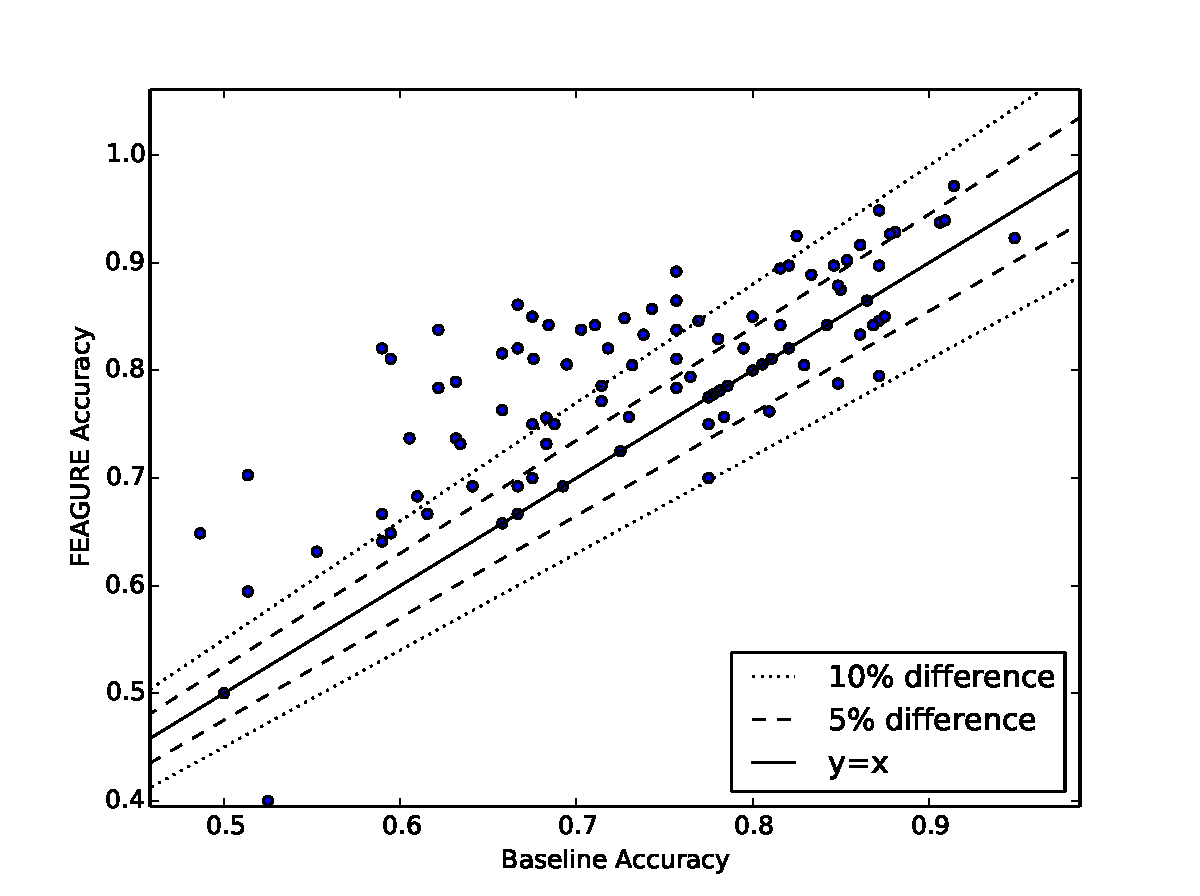
\includegraphics[width=1.2\textwidth]{svm_full} % first figure itself
		\caption{Accuracy of
			baseline approach compared to one-level activation of \emph{FEAGURE} (SVM). Each point represents a dataset. The dotted lines represent a 5 and 10 percent difference in accuracy}
		\label{fig:svm_base_lvl1}
	\end{minipage}\hfill
	\begin{minipage}{0.45\textwidth}
		\centering
		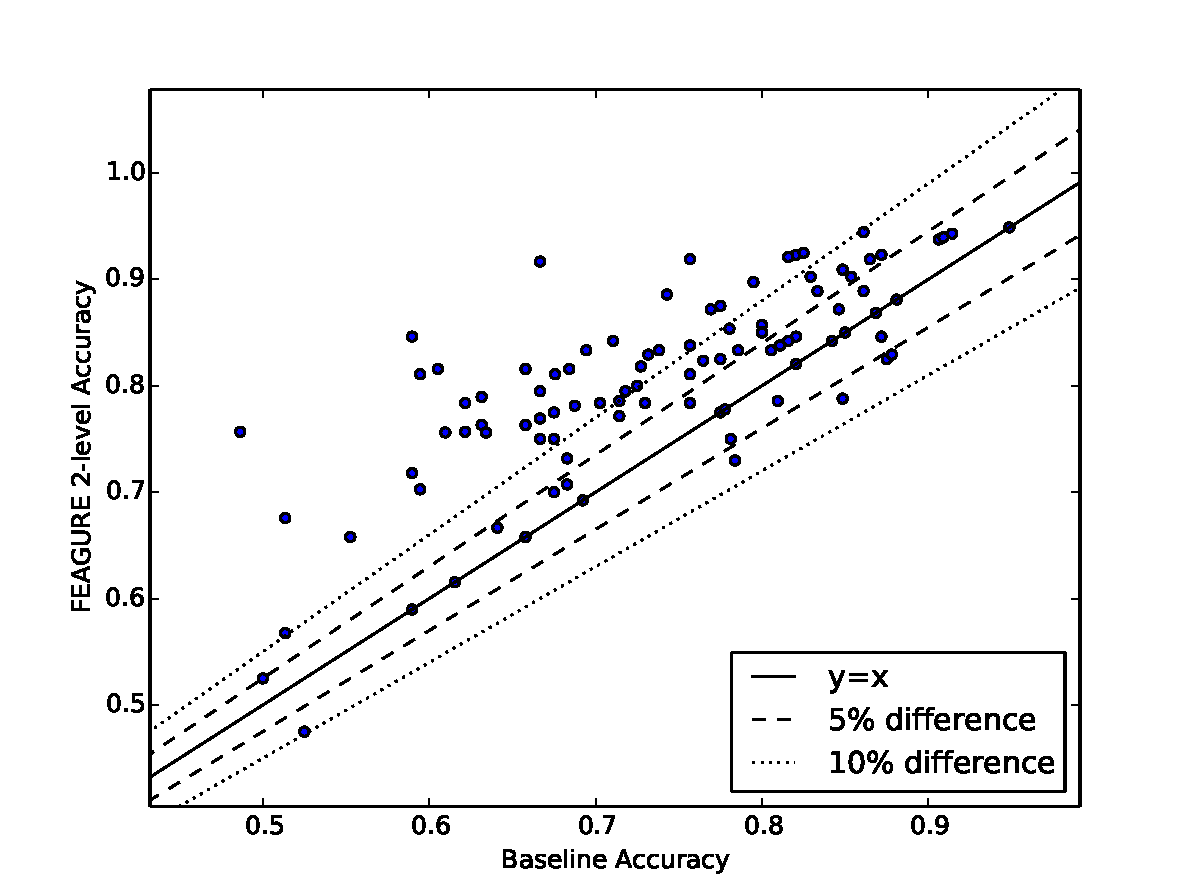
\includegraphics[width=1.2\textwidth]{svm_full_lvl2} % second figure itself
		\caption{Accuracy of
			baseline approach compared to two-level activation of \emph{FEAGURE} (SVM). Each point represents a dataset. The dotted lines represent a 5 and 10 percent difference in accuracy}
		\label{fig:svm_base_lvl2}
	\end{minipage}
\end{figure}


In their paper on TechTC-100, \citeA{gabrilovich2004text} define a metric called Maximal Achievable Accuracy (MAA). This criterion attempts to assess the difficulty of the induction problem by the maximal ten-fold accuracy over three very different induction algorithms (SVM, K-NN and CART).
%Intuitively, a dataset with low MAA can be considered harder than one with a high MAA. %, since a known induction algorithm can achieve a higher accuracy for the dataset with higher MAA. needs to be better justified(one strong == easy)
Figure \ref{fig:25best} shows the performance of \emph{FEAGURE} on the 25 hardest datasets in TechTC-100, in terms of the MAA criterion. We call this dataset collection ``TechTC-25MAA." 
Table \ref{table:acc} shows the accuracies for the 25 hardest datasets in TechTC-100, in terms of the MAA criterion. We call this dataset collection ``TechTC-25MAA." 
These results show a much more pronounced increase in accuracy, and illustrate that we can, in general, rely on \emph{FEAGURE} to yield positive features for difficult classification problems.

\begin{table}[!h]
	\centering
	\caption{Average accuracy over the 25 hardest datasets in terms of MAA. The columns specify the feature generation approach, with the baseline being no feature generation. The rows specify the induction algorithm used on the generated features for evaluation. Best results are marked in bold.}
	\label{table:acc_maa}
	\begin{tabular}{|l | l || l | l | l| l|}
		\hline
		Dataset & Classifier & Baseline   & Expander-FG & FEAGURE   & FEAGURE 2-level    \\ \hline
		
		\multirow{3}{*}{TechTC-25MAA} & KNN & 0.524 & 0.723 ($p<0.001$) & \textbf{0.803 ($p<0.001$)} & 0.795 ($p<0.001$)  \\ \cline{2-6}
		
		& SVM  & 0.751 & 0.815 ($p<0.001$)    & 0.817 ($p<0.001$)    & \textbf{0.829 ($p<0.001$)} \\ \cline{2-6}
		
		& CART  & 0.82 & 0.839   & 0.837   & \textbf{0.849 ($p<0.05$)}  \\
		
		\specialrule{.15em}{.05em}{.01em}
		
		\multirow{3}{*}{TechTC-100} & KNN & 0.531 & 0.702 ($p<0.001$) & 0.772 ($p<0.001$) & \textbf{0.775 ($p<0.001$)}  \\ \cline{2-6}
		& SVM  & 0.739 & 0.782 ($p<0.001$)    & 0.796 ($p<0.001$)    & \textbf{0.807 ($p<0.001$)} \\ \cline{2-6}
		
		& CART  & 0.81 & 0.815   & 0.814   & \textbf{0.825 ($p<0.05$)}  \\
		
		\specialrule{.15em}{.05em}{.01em}
		
	\end{tabular}
\end{table}

\begin{figure}
	\centering
	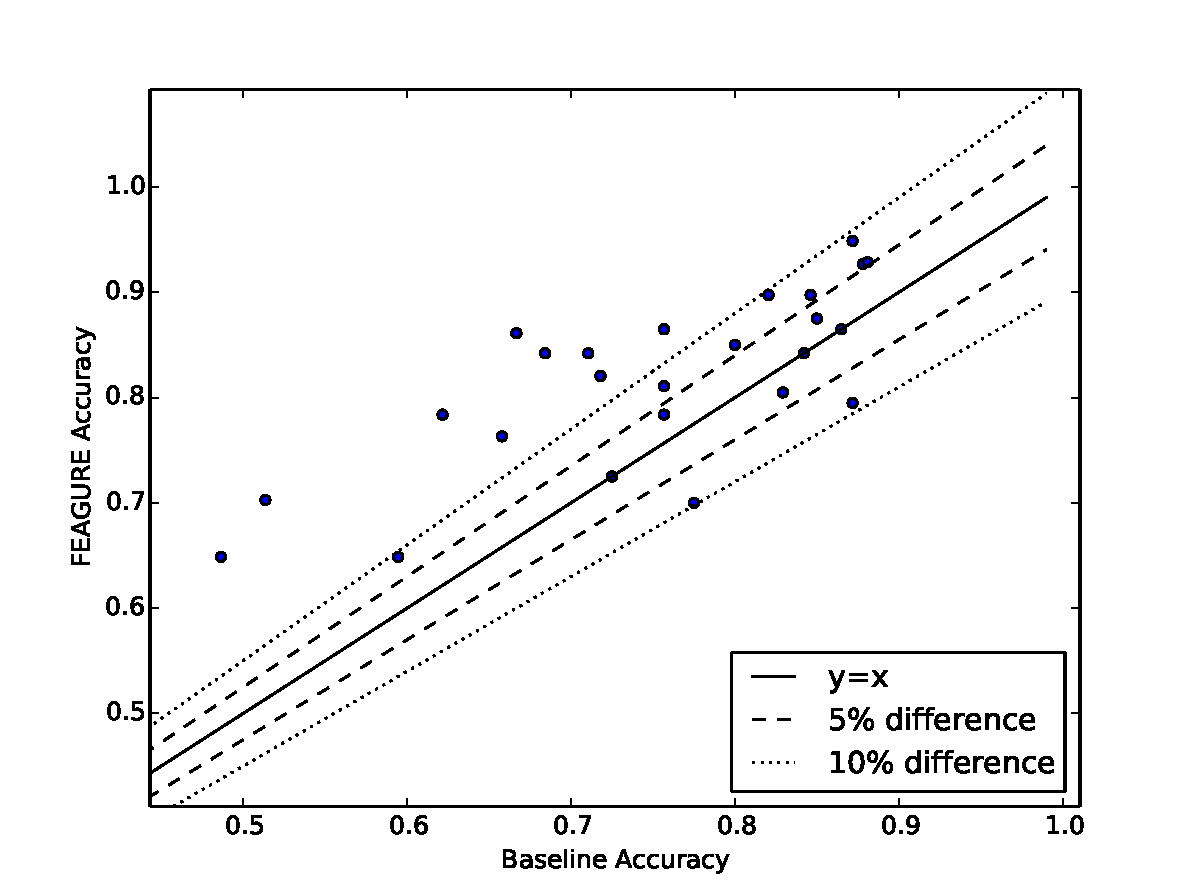
\includegraphics[width=0.8\linewidth]{25best}
	\caption{Accuracy of the
		baseline approach compared to single-level activation of \emph{FEAGURE} (SVM). Displayed are the 25 hardest datasets (those with the lowest MAA)}
	\label{fig:25best}
\end{figure}

%\subsection{Effect of recursive problem classifier on \emph{FEAGURE}}

As discussed in Section \ref{algorithm_section}, \emph{FEAGURE} creates a generic learning problem as part of its execution. For our main results we learned a decision tree classifier for this new induction problem.
We also tested the effects of using K-NN and SVM classifiers instead. %, with the following parameters: For K-NN, we used $K=3$. For SVM we used $C=10$, with both Linear and a Radial Basis Function (RBF) kernels.
We note that this choice is orthogonal to that of the induction algorithm used to evaluate the generated features.

Table \ref{table:acc-nontree} shows the accuracies achieved with these induction algorithms. We see that in general, with the exception of an external K-NN classifier that uses an internal RBF-SVM, replacing the internal tree induction algorithm does not increase the accuracy of the resulting feature map.

\begin{table*}[!th]
	\centering
	\caption{Average accuracy over all datasets. The columns specify the induction algorithm used in \emph{FEAGURE} (SVM with linear or RBF kernel, K-NN). The rows specify the induction algorithm used on the generated features for evaluation. Entries marked with * show a statistically significant p-value over the baseline accuracy.}
	\label{table:acc-nontree}
	\centering
	\begin{tabular}{|l | l || l || l | l| l|l|}
		\hline
		Dataset & Classifier  & Baseline & Expander-FG & Tree  & RBF SVM & 5-NN    \\ \hline
		
		\multirow{3}{*}{OHSUMED} & KNN  & 0.777 & 0.756 & 0.769 & \textbf{0.795*}   & 0.771 \\ \cline{2-7}
		& SVM  & 0.797 & 0.804 & \textbf{0.816*}   & 0.796    & 0.788 \\ \cline{2-7}
		
		& CART  & 0.806 & \textbf{0.814} & 0.809   & 0.791    & 0.787 \\
		
		\specialrule{.15em}{.05em}{.01em} % \hline
		
		\multirow{3}{*}{TechTC-100} & KNN & 0.531 & 0.702* & \textbf{0.772*} & 0.689*   & 0.705*\\ \cline{2-7}
		& SVM   & 0.739 & 0.782* & \textbf{0.796*}  & 0.774*   & 0.774* \\ \cline{2-7}
		
		& CART & 0.81 & \textbf{0.815} & 0.814   & 0.81    & 0.79 \\
		
		\specialrule{.15em}{.05em}{.01em} % \hline
		
		%\multirow{3}{*}{TechTC-25H} & KNN & 0.524 & 0.723* & \textbf{0.803*} & 0.744* & 0.7239*   & 0.724*\\ \cline{2-8}
		%& SVM   & 0.751 & 0.815* & \textbf{0.817*} & 0.794*  & 0.799*   & 0.782* \\ \cline{2-8}
		
		%& CART & 0.82 & \textbf{0.839} & 0.837 & 0.786   & 0.799    & 0.801 \\
		
		%\specialrule{.15em}{.05em}{.01em} % \hline
		
	\end{tabular}
\end{table*}

\subsection{Quantitative Analysis}

%we must first try to better understand its output and how it behaves from a variety of angles.
%In this section, we examine the following factors:
%\begin{enumerate}
%	\item Number of features tried during the feature generation process compared number of features generated
%	\item Number of features generated per depth of the divide \& conquer process
%	\item Size of new induction problems relative to existing ones
%	\item Local Information gain of generated features
%\end{enumerate}

To better understand the behavior of the \emph{Deep-FEAGURE} algorithm, we measured its output and performed several aggregations over it.
We first look at the average number of features considered by \emph{Deep-FEAGURE} at every node: for TechTC-100, out of an average of 36.7 partitions by type that are considered for each feature, an average of 7.3 are expanded into new features by \emph{FEAGURE}. The rest of the generated problems are discarded due to the filtering criteria mentioned in Section \ref{code-tree-thing}.
We note that there are 46 available relations, and thus we can expect to look at no more than 46 features (if a relation does not apply to a sub-problem, it is not counted in this average). 

When the depth of the search tree increases, the number of generated features decreases rapidly, as shown in Figure \ref{fig:features_per_depth}.
This is unsurprising, as we know that increased depth will cause generated problems to have a smaller training set, increasing the likelihood of those features to be filtered out. Additionally, we see that the number of available features decreases in a roughly linear manner with depth. This is again unsurprising, as features deeper in the tree cannot easily make use of the same relation multiple times due to the orthogonality trait discussed in Section \ref{tree_usage}.

\begin{figure}[h!]
	\centering
	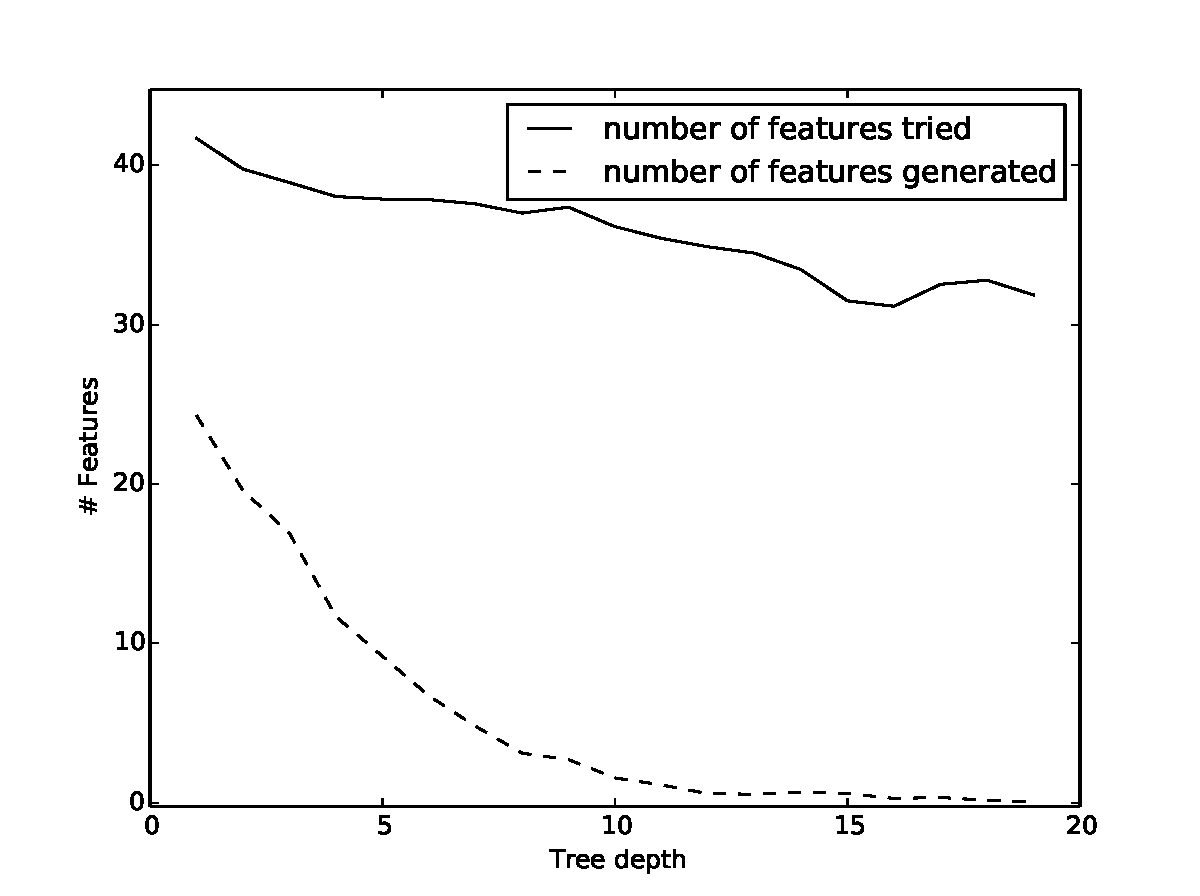
\includegraphics[scale=0.4]{features_per_depth}
	\caption{Average number of features tried vs. average number of features generated per depth.}
	\label{fig:features_per_depth}
\end{figure}

%An interesting measure with regards to the newly constructed features is that of relative information gain, compared to existing features. Table \ref{table:ig_errorbars} shows the mean and standard deviation in information gain. We see that compared to word-based features, the features generated by \emph{FEAGURE} are better on average, with a much higher standard deviation, indicating more variance in terms of information gain. When looking at these information gains split by depth, we see that this high variance is mostly due to features created deeper in the search process.

%\begin{table}[]
%	\centering
%	\caption{Mean IG and standard deviation for features generated by \
%emph{FEAGURE} compared to baseline features.}
%	\label{table:ig_errorbars}
%	\centering
%	\begin{tabular}{|l || l | l|}
%		\hline
%		Feature set & Mean IG  & Standard deviation  \\ \hline
%		Baseline  & 0.01 & 0.015 \\
%		\hline
%		FEAGURE & 0.025 & 0.05 \\
%		\hline 
%	\end{tabular}
%\end{table}

Let us now compare the relative size of recursive problems to the existing induction problems. Figure \ref{fig:problem_ratio} shows the ratio between the number of examples (size) in the  newly constructed induction problem and the size of the original learning problem at various depths of the divide \& conquer search process. 
As depth in the search tree increases, the size ratio increases as well. This is somewhat surprising, as an increase in depth means a smaller induction problem, and thus we would expect a similar size ratio to be maintained. Even more unexpected, however, is that the average \textbf{recursive} problem size increases with problem depth. Intuitively, we would have expected the recursive problem size to decrease as problem depth increases. However, as we search smaller problems deeper down the search process, the relations that result in a smaller or roughly similar sized recursive induction problem have already been used, and thus relations that cause a larger size ratio are required.

We also note that these recursive problems do not maintain the same label balance as the original learning problems: one label set is much larger. This is expected, as the divide \& conquer search strategy aims to use the label set as a basis for separation. We may therefore wish to make use of various known strategies to reduce the impact of label imbalance in induction problems when using \emph{Deep-FEAGURE}.

\begin{figure}[h!]
	\centering
	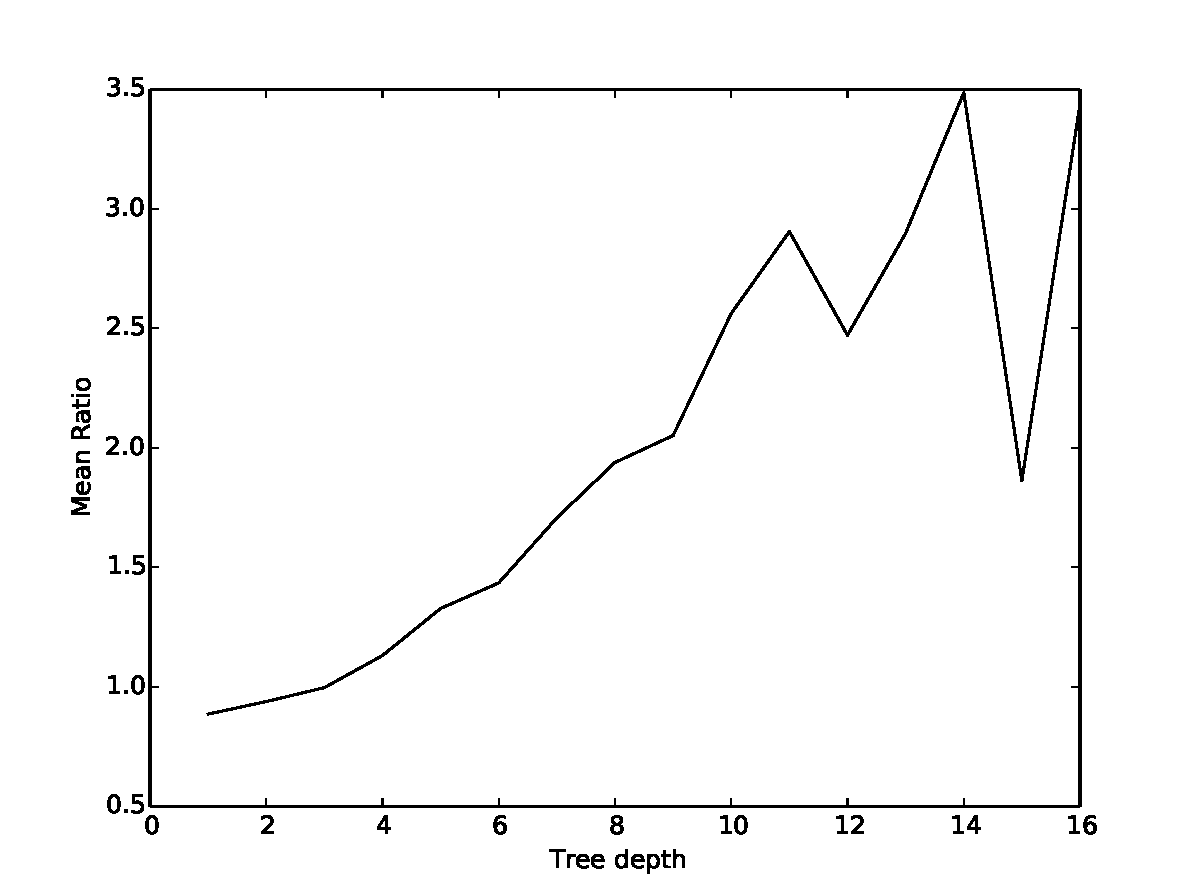
\includegraphics[scale=0.4]{problem_ratio}
	\caption{Mean size ratio of newly created recursive problem compared to the original learning problem size (new problem training set size divided by original problem training set size).}
	\label{fig:problem_ratio}
\end{figure}

Finally, we look at the local information gain of the newly created features. In Figure \ref{fig:local_ig_depth}, we see the mean information gain of generated features per depth, compared to the best information gain achieved by a non-recursive feature for that depth. We see that our recursive features tend to have a much higher information gain, especially in the beginning of the search process. We see a decrease in both measures as depth increases, because it is then more difficult to find distinguishing features.

\begin{figure}[h!]
	\centering
	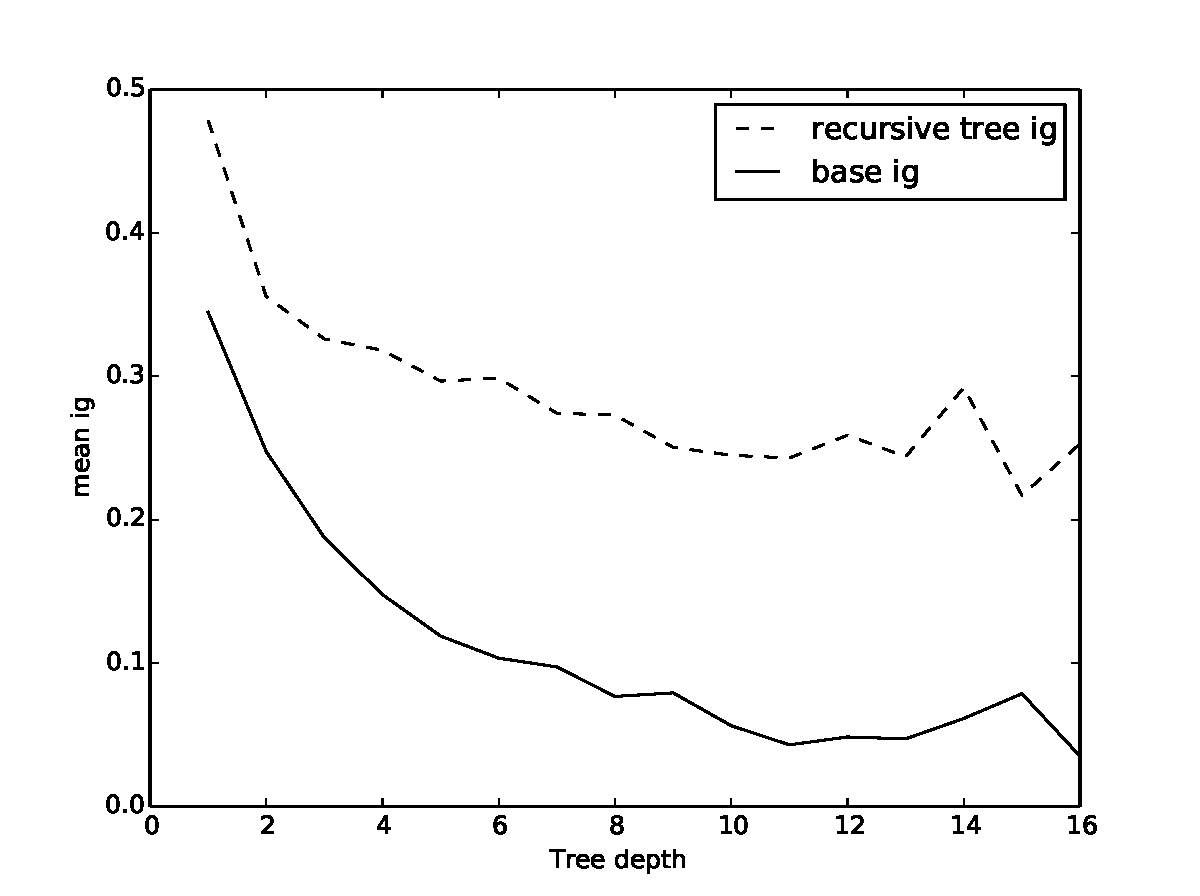
\includegraphics[scale=0.4]{local_ig_depth}
	\caption{Mean information gain of generated features compared to the best information gain for the original learning problem.}
	\label{fig:local_ig_depth}
\end{figure}

\subsection{Qualitative Analysis}

To better understand the contribution of the features constructed by \emph{FEAGURE}, let us look at a few generated features. We will consider the output of our algorithm on datasets from the TechTC-100 collection.

\subsubsection{A simple example}

For our first example, let us consider a single-level feature construction.
In this example, we are attempting to separate texts regarding Virginia businesses from those discussing locations in Michigan. Early in the learning process, we apply \emph{FEAGURE} to this problem, taking entities from the texts. We create a recursive problem over the subset of entities contained in the domain of the ``owns" relation (most of which are organizations). Thus, this new problem (Figure \ref{fig:figure_rec1_example}) attempts to separate organizations mentioned in texts regarding Virginia businesses from those mentioned in texts regarding locations in Michigan.

\begin{figure}[!h]
	\centering
	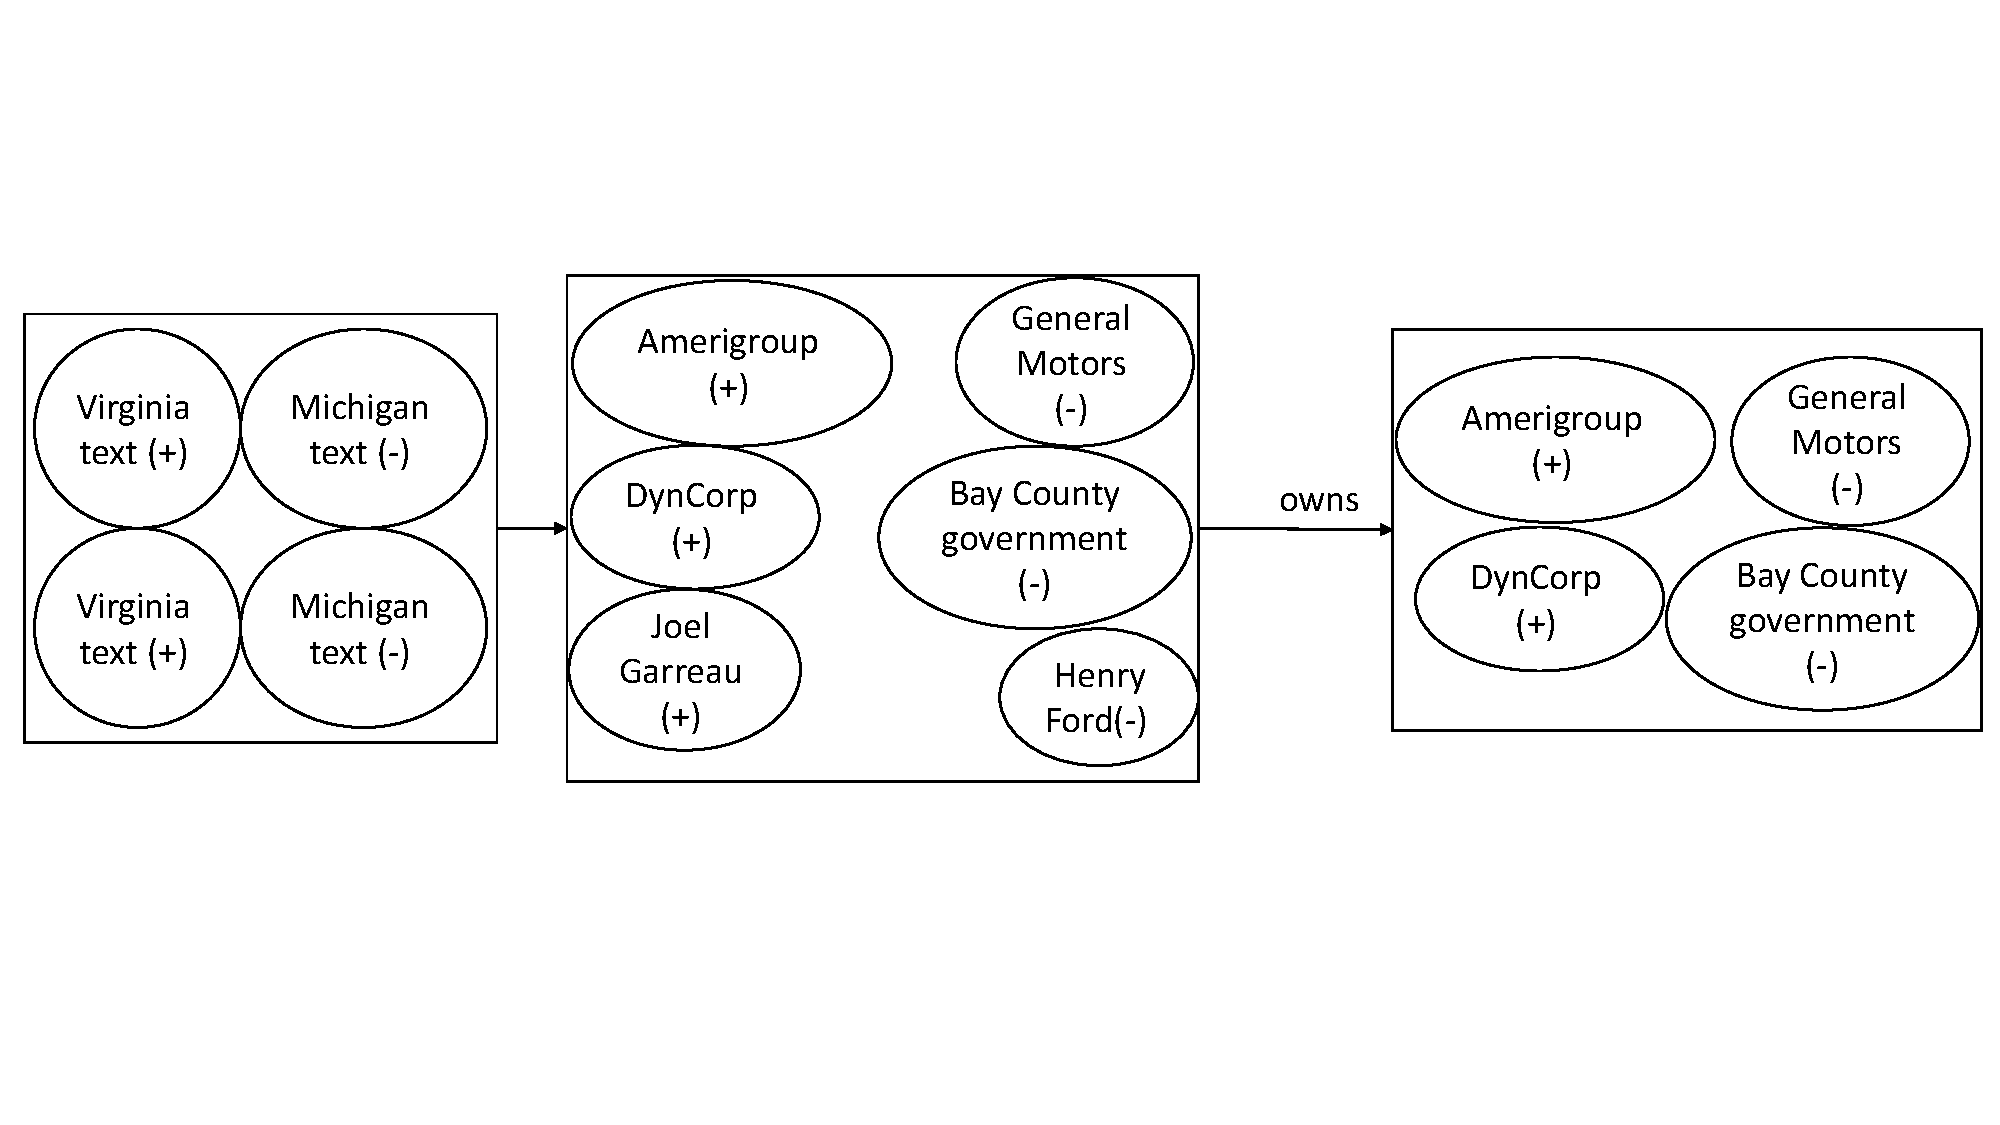
\includegraphics[width=\linewidth]{figure_rec1_example_new}
	\caption{The left box represents the original learning problem. The middle box shows the entities extracted from the original problem. The right box represents the new learning problem containing entities that serve as keys for a specific relation.}
	\label{fig:figure_rec1_example}
\end{figure}

\begin{figure}[!h]
	\centering
	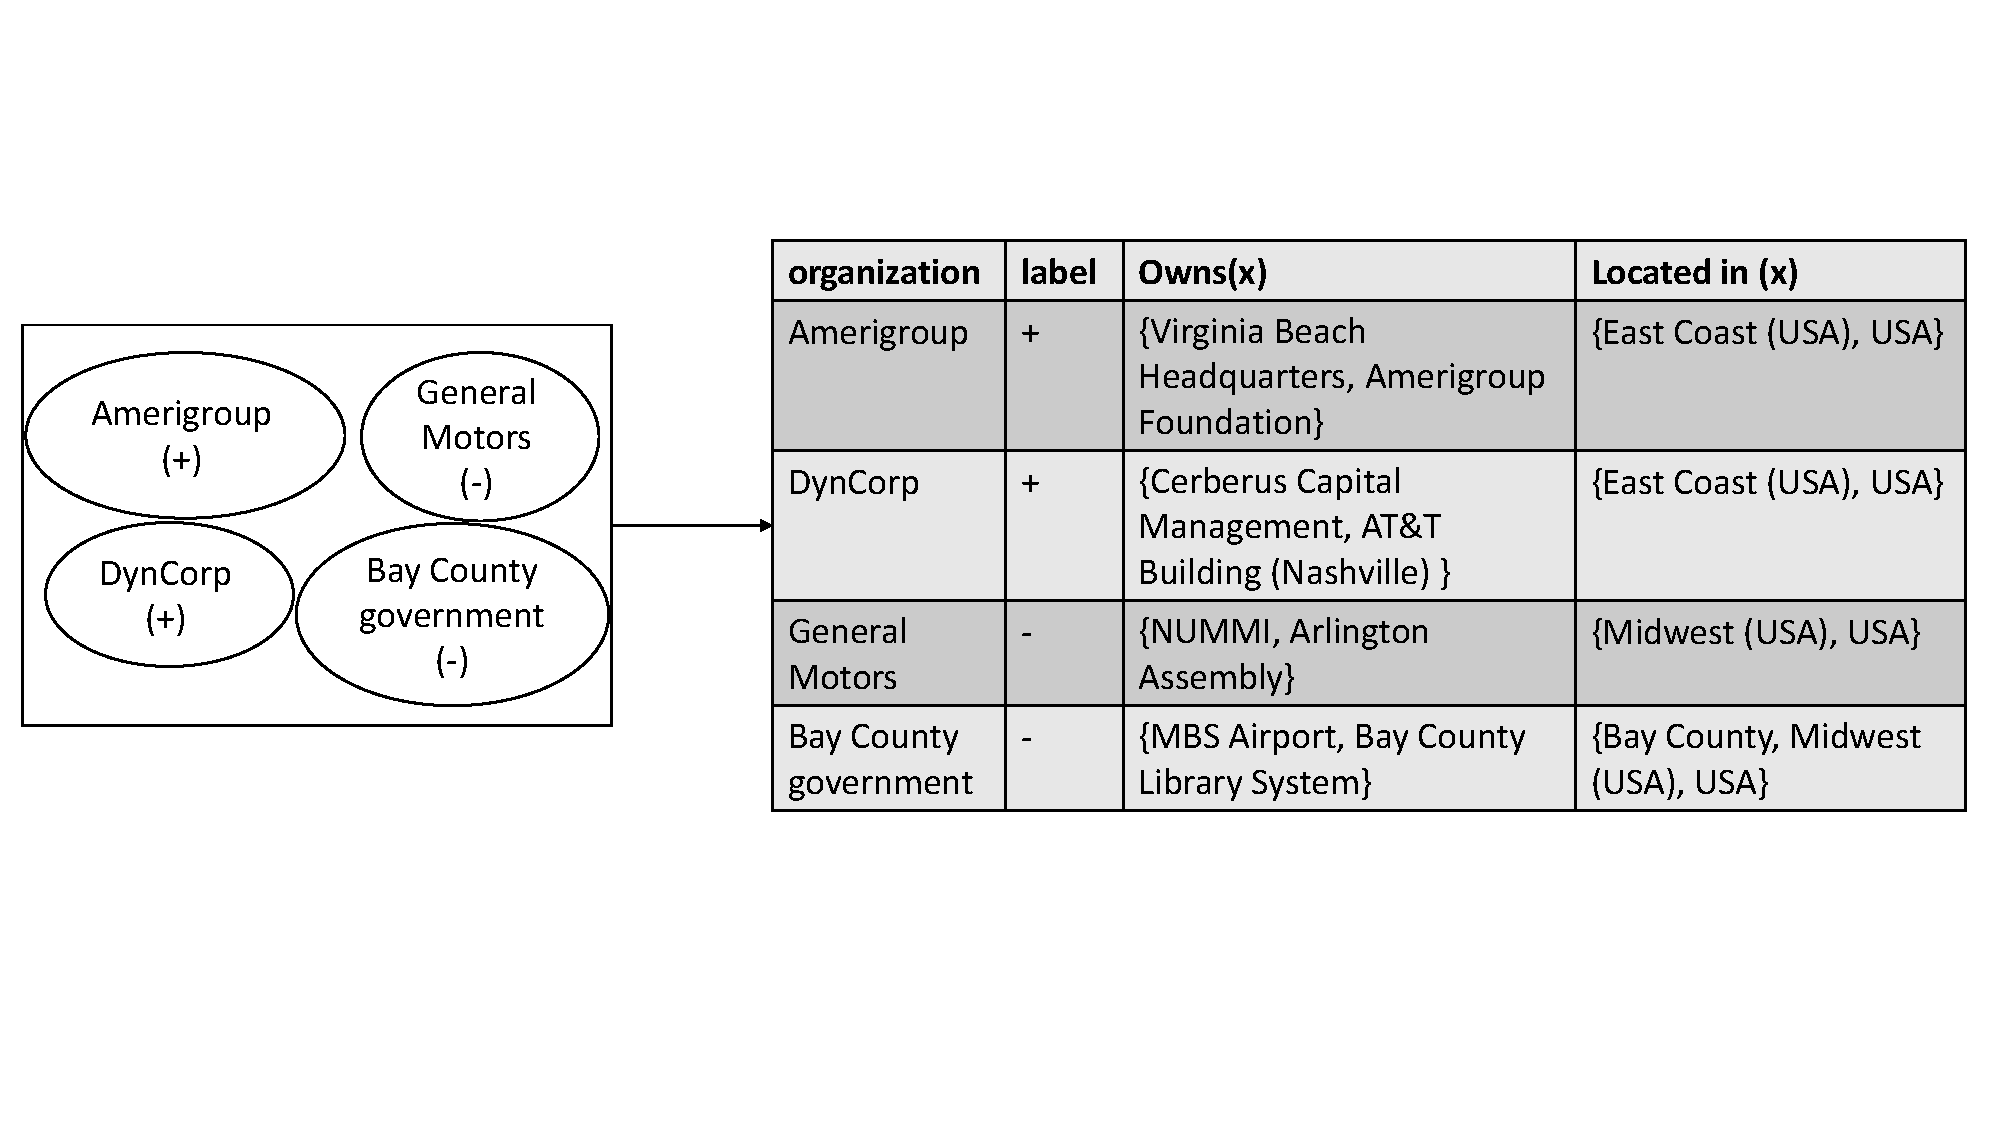
\includegraphics[width=\linewidth]{figure_rec1_problem_new}
	\caption{Recursive induction problem creation process: Features are created using the relational knowledge base.}
	\label{fig:figure_rec1_problem}
\end{figure}

At this stage, our algorithm has constructed a new learning problem, whose objects are organizations, labeled by the original learning problem. 
In the next step, the algorithm uses applicable relations, the ``Owns" and ``Located in" relations in this case, to convert the objects to feature vectors.
Since an organization can own more than one property, and can be located in more than one location, these two features have multi-valued attributes. Figure \ref{fig:figure_rec1_problem} shows the resulting labeled feature vectors.
This new learning problem is fed as input to an induction algorithm (in this case, a decision tree learner), resulting in the classifier shown in Figure \ref{fig:feature_eastcoast_rel}. This classifier is used as a binary feature in the original domain, representing the concept of organizations located in the East Coast region of the United States.
This is a powerful feature, as Virginia is an East Coast state, whereas Michigan is not. Therefore, texts regarding Virginia businesses are significantly more likely to link to organizations located on the East Coast than are texts regarding Michigan. We note that this particular feature was indeed generated by our algorithm and was later used by our external induction algorithm due to its high information gain.
%This generalization is mostly achieved by the expressiveness of the relation knowledge base, and the fact that the ``located in" relation offers a combination of narrow and broad regions.

\begin{figure}[!h]
	\centering
	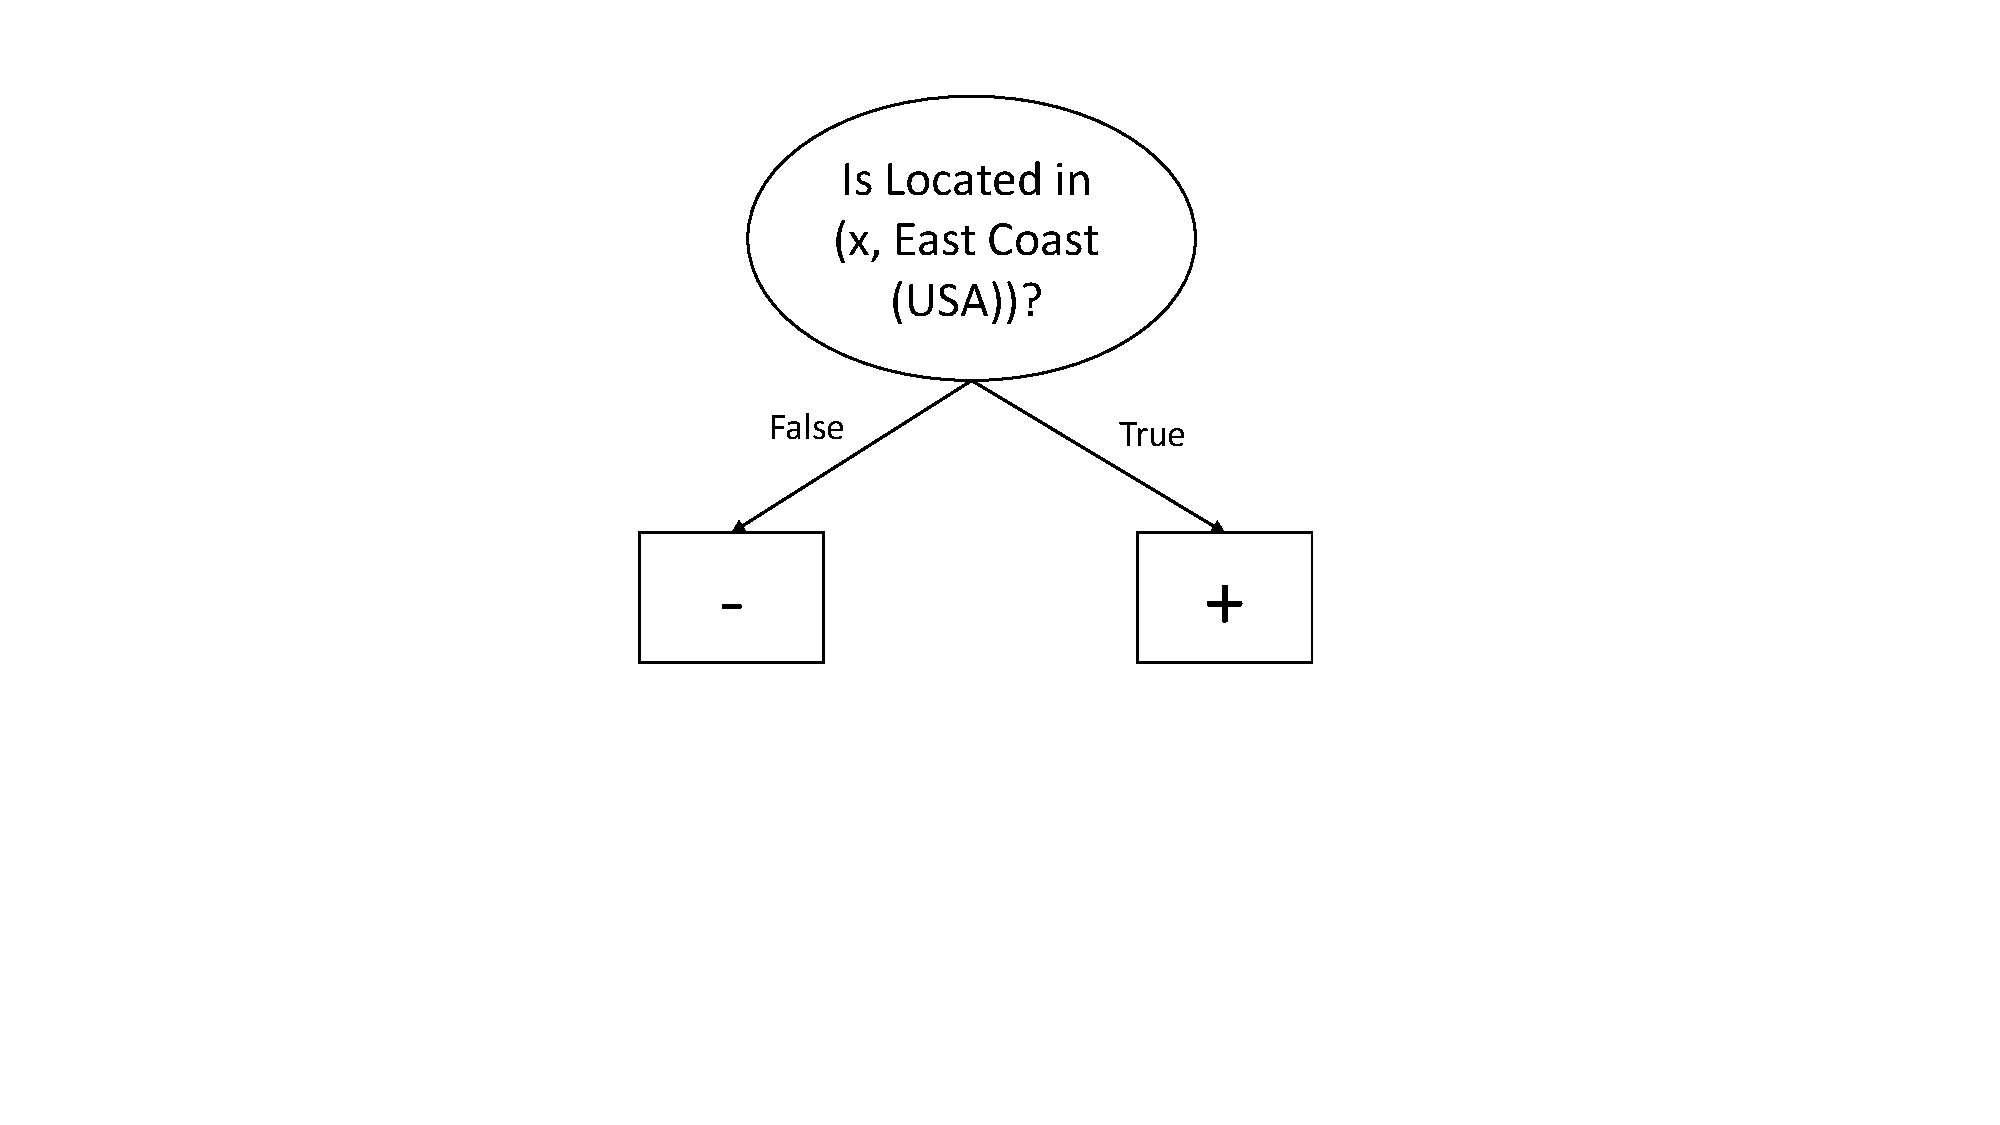
\includegraphics[width=0.5\linewidth]{figure_rec1_feature_new}
	\caption{Feature constructed by \emph{FEAGURE} for entities (organisations) in the ``owns" relation.}
	\label{fig:feature_eastcoast_rel}
\end{figure}

\subsubsection{A more complex example}

Our next example shows a slightly more complex feature within a single-level activation of \emph{FEAGURE}. Here, we are attempting to separate texts that pertain to locations in California from those that pertain to locations in Alabama. 
Once again, entities are extracted, and this time, we take the subset of entities in the domain of the ``lives in" relation. The resulting entities are people labeled according to the original tagging (Figure \ref{fig:figure_rec2_example}).
To create a classifier for this problem, our algorithm uses all applicable relations (``Type", ``Citizen of" and ``Died in") to create features for the newly created induction problem. %separating people mentioned in texts regarding California locations from people mentioned in texts regarding Alabama locations.
This process is demonstrated in Figure \ref{fig:figure_rec2_problem}.

\begin{figure}[!h]
	\centering
	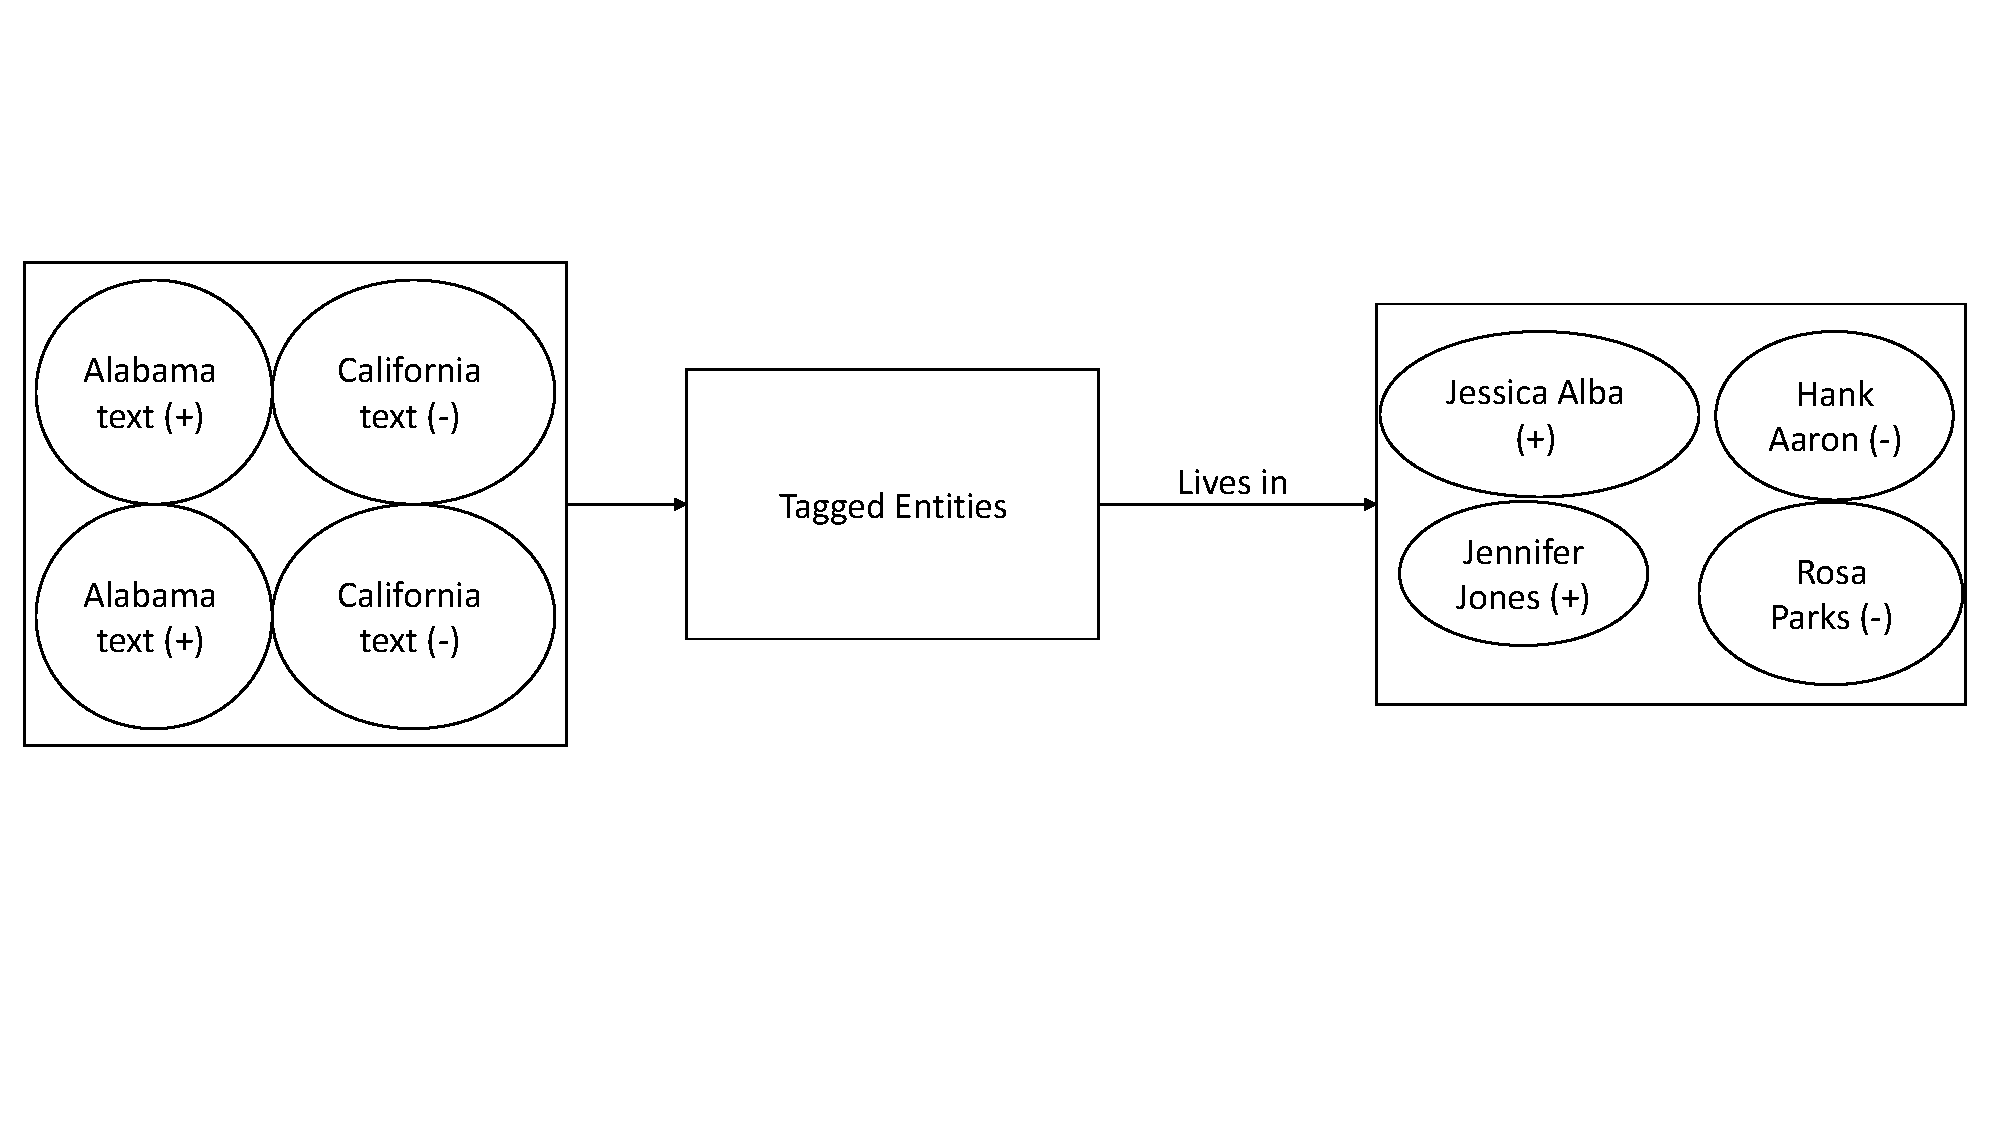
\includegraphics[width=\linewidth]{figure_rec2_example_new}
	\caption{Entities are extracted and labeled. These entities are the new example set. The left box shows the original learning problem. The middle box represents entities extracted from the problem. The right box shows the new learning problem containing a subset of entities in a single domain.}
	\label{fig:figure_rec2_example}
\end{figure}

\begin{figure}[!h]
	\centering
	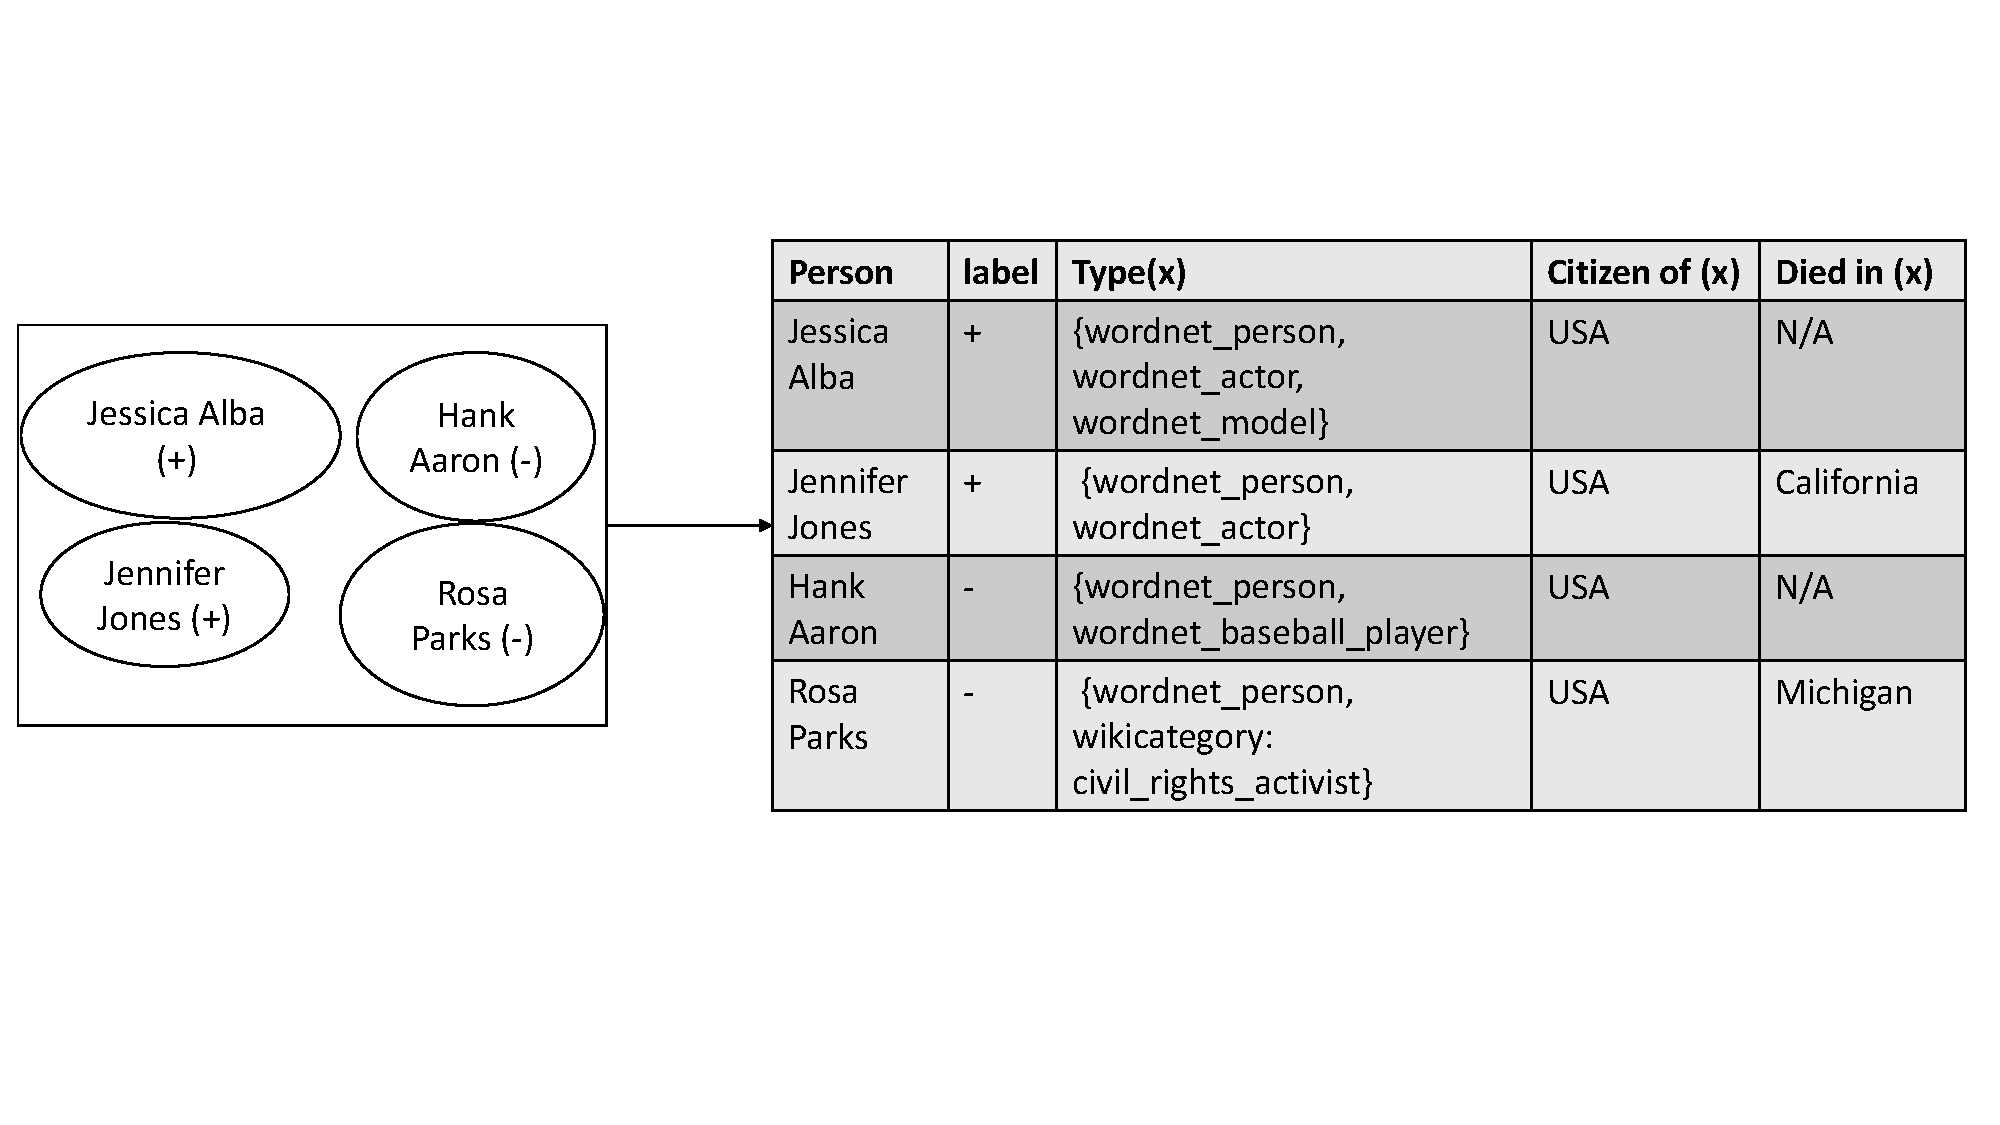
\includegraphics[width=\linewidth]{figure_rec2_problem_new}
	\caption{Applicable relations are used as feature function for the new example set.}
	\label{fig:figure_rec2_problem}
\end{figure}


Once this recursive learning problem has been constructed, our algorithm induces a decision tree classifier for it, yielding the recursive feature described in Figure \ref{fig:figure_rec2_feature}. This feature is then applied as a binary feature for people in the text, and can be described as ``is this person an actor, director or model?".
This feature is quite useful, as a person living in California is much more likely to belong to one of these categories than someone living in Alabama. This feature shows how type relations (also known as ``is-a" relations or hypernyms) can be used to effectively group together several types of celebrity figures, namely actors, directors and models.

\begin{figure}[h!]
	\centering
	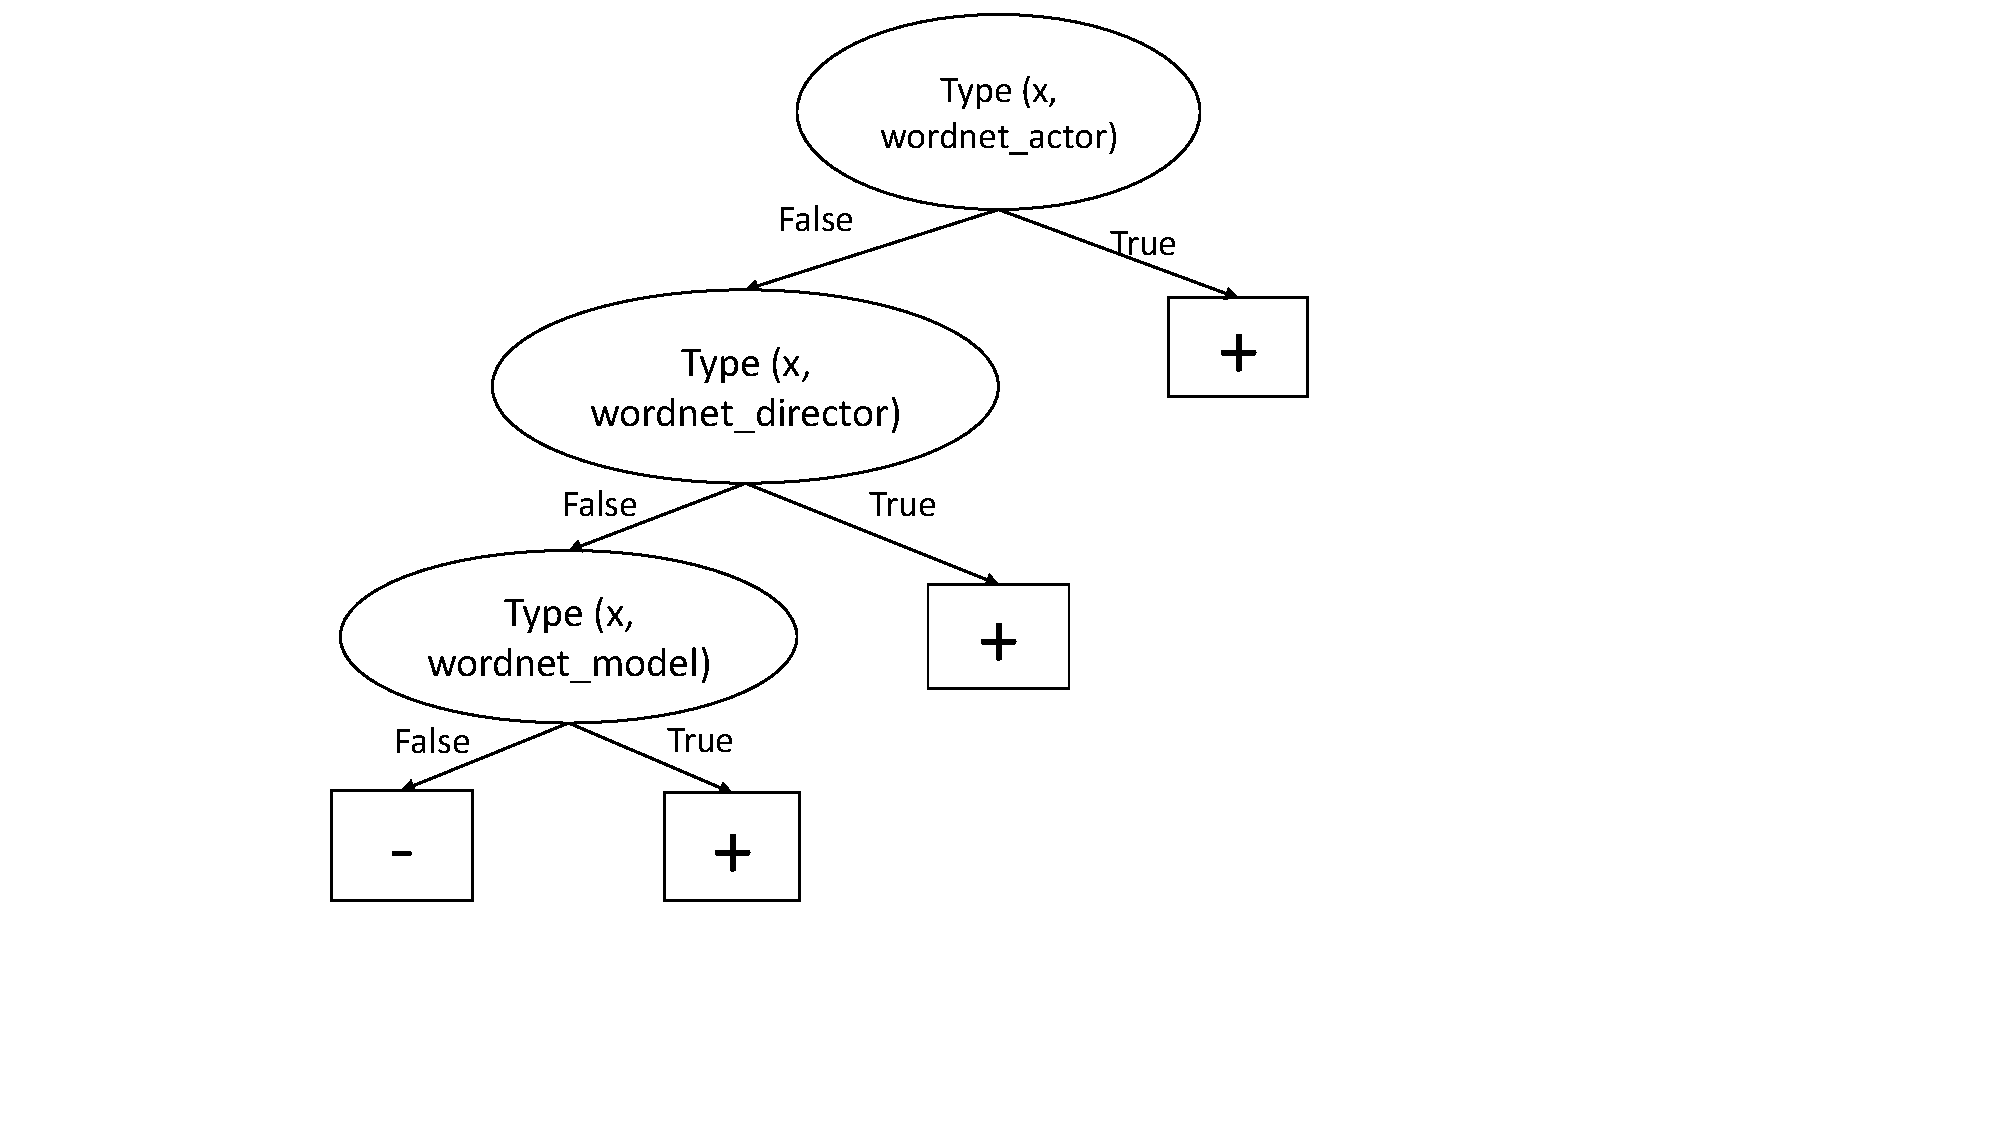
\includegraphics[width=0.7\linewidth]{figure_rec2_feature_new}
	\caption{Feature constructed by FEAGURE for entities (people) in the ``lives in" relation.}
	\label{fig:figure_rec2_feature}
\end{figure}

\subsubsection{Recursive application of \emph{FEAGURE}}

In this example, texts refer either to locations in and around Texas, or to locations in and around New York. As before, entities are extracted and labeled. This time, locations are our entities, with the ``Located in" relation as our domain (Figure \ref{fig:figure_rec3_example}). Applicable relations are used to then create a new induction problem. \emph{FEAGURE} uses the ``Located in" and ``Happened in" relations as features for this problem, as shown in Figure \ref{fig:figure_rec3_problem}. 

\begin{figure}[!h]
	\centering
	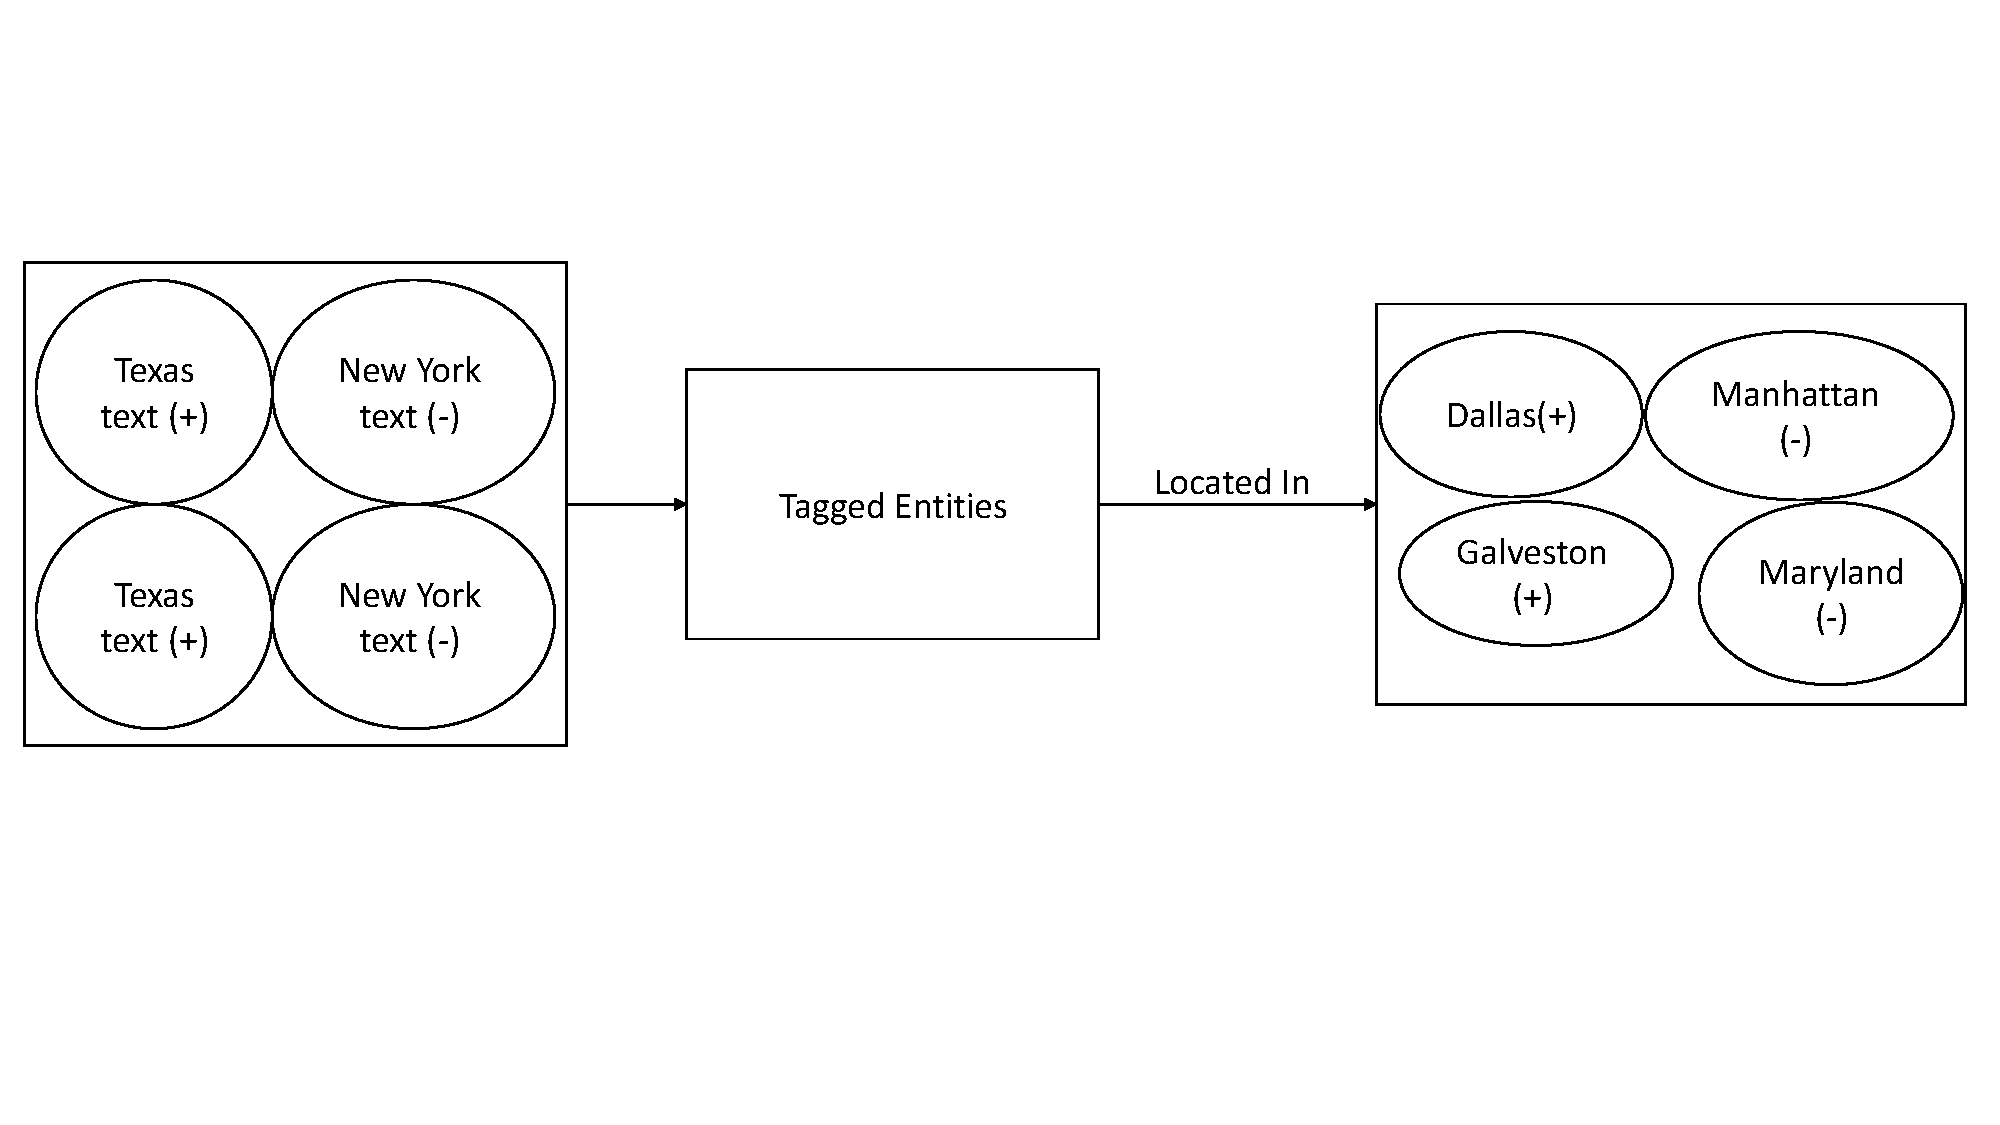
\includegraphics[width=\linewidth]{figure_rec3_example_new}
	\caption{Entities are extracted from the text, and entities in the ``Located in" relation are used as labeled objects.}
	\label{fig:figure_rec3_example}
\end{figure}

\begin{figure}[!h]
	\centering
	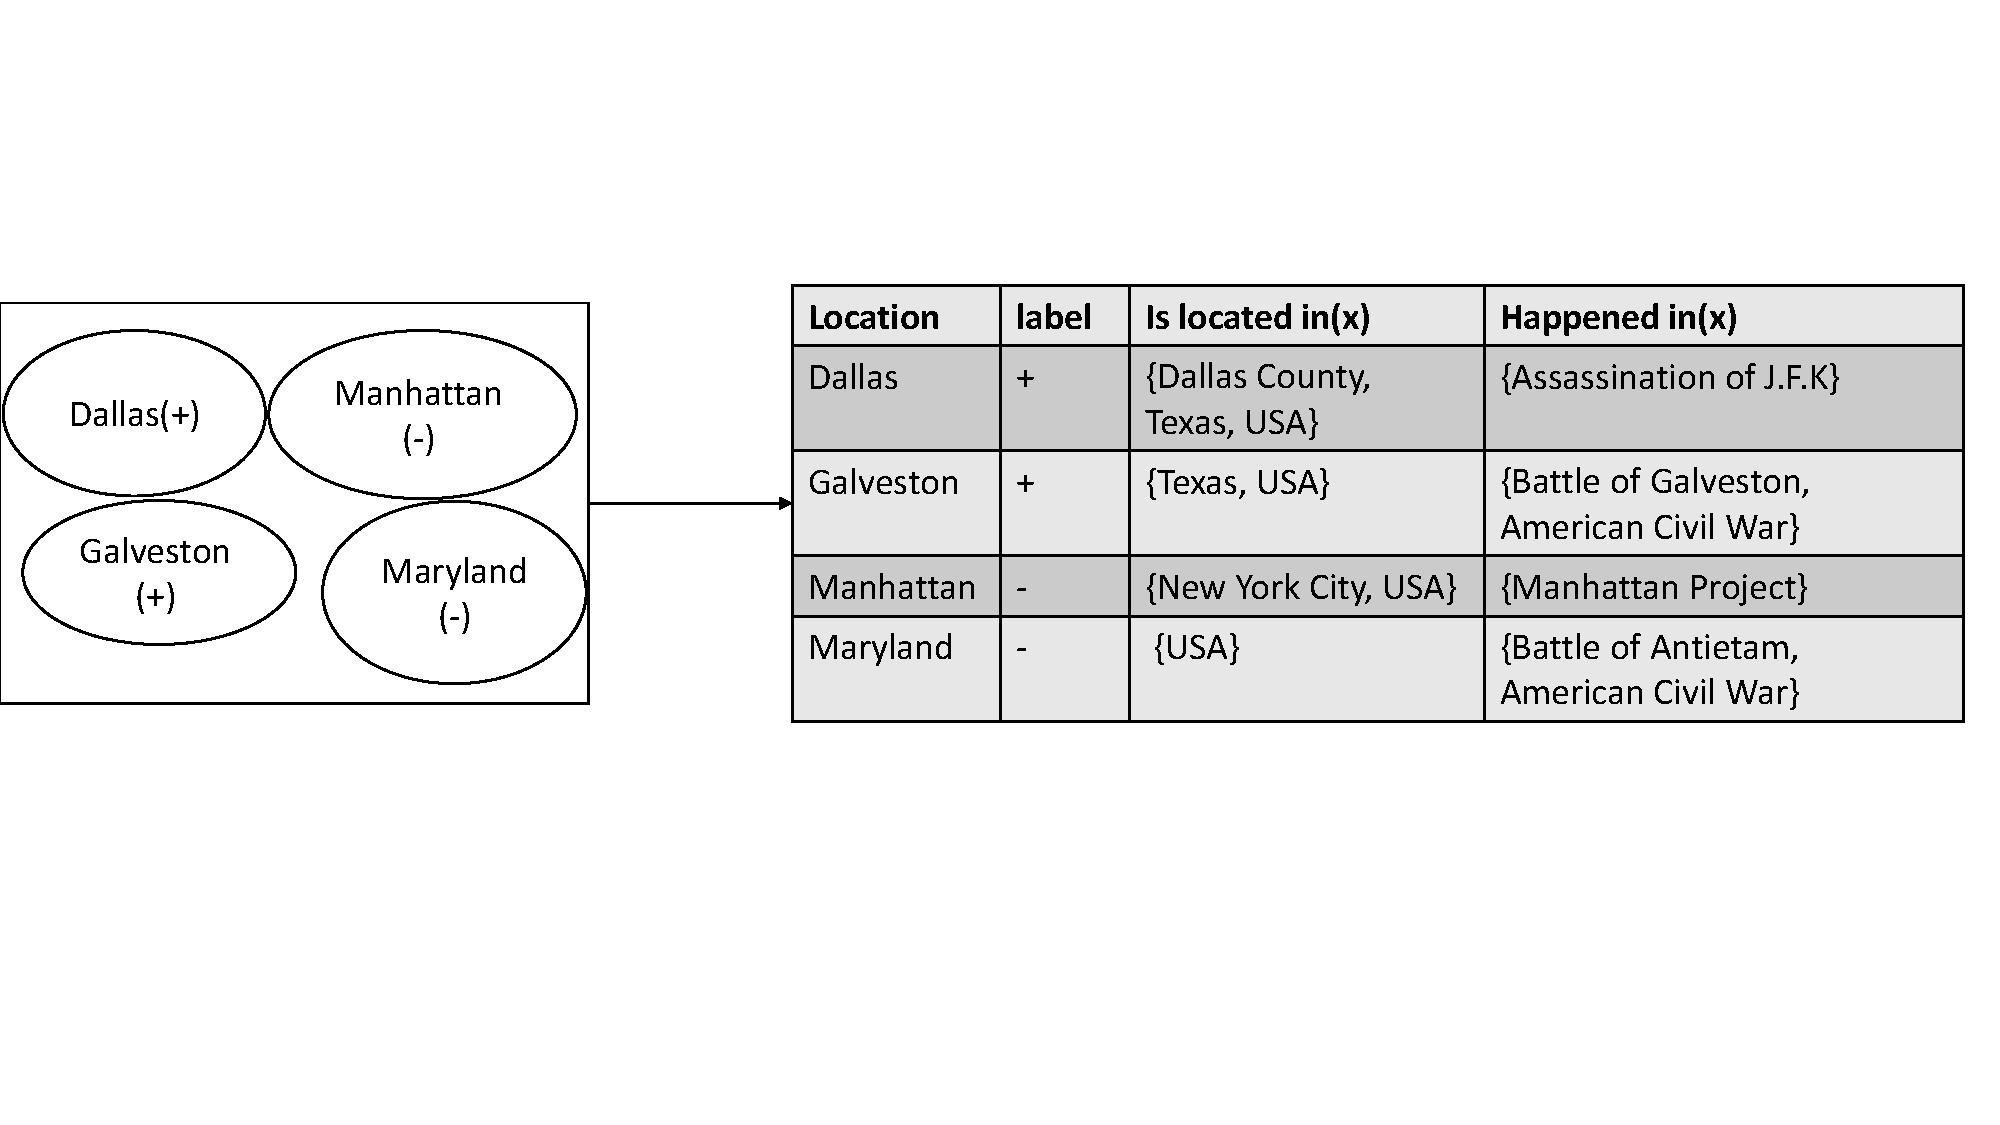
\includegraphics[width=\linewidth]{figure_rec3_problem_new}
	\caption{Construction of a recursive learning problem based on the ``Located in" relation. Applicable relations are used to create a feature set for the newly constructed example set.}
	\label{fig:figure_rec3_problem}
\end{figure}

This feature set is not sufficient for creating a good classifier for our learning problem. Therefore, the algorithm calls \emph{FEAGURE} recursively to try and generate new features for the new induction problem.
The values of the feature ``Happened in" are events. These events are used as objects for a recursive learning problem (Figure \ref{fig:figure_rec3_example_rec}).
We use the ``Type" relation as a feature, relying on hypernyms to classify events (Figure \ref{fig:figure_rec3_problem_rec}).
The resulting classifier (a decision tree induction algorithm was used) is shown in Figure \ref{fig:figure_rec3_feature}, and can be interpreted as ``is this event a battle or conflict?".

\begin{figure}[!h]
	\centering
	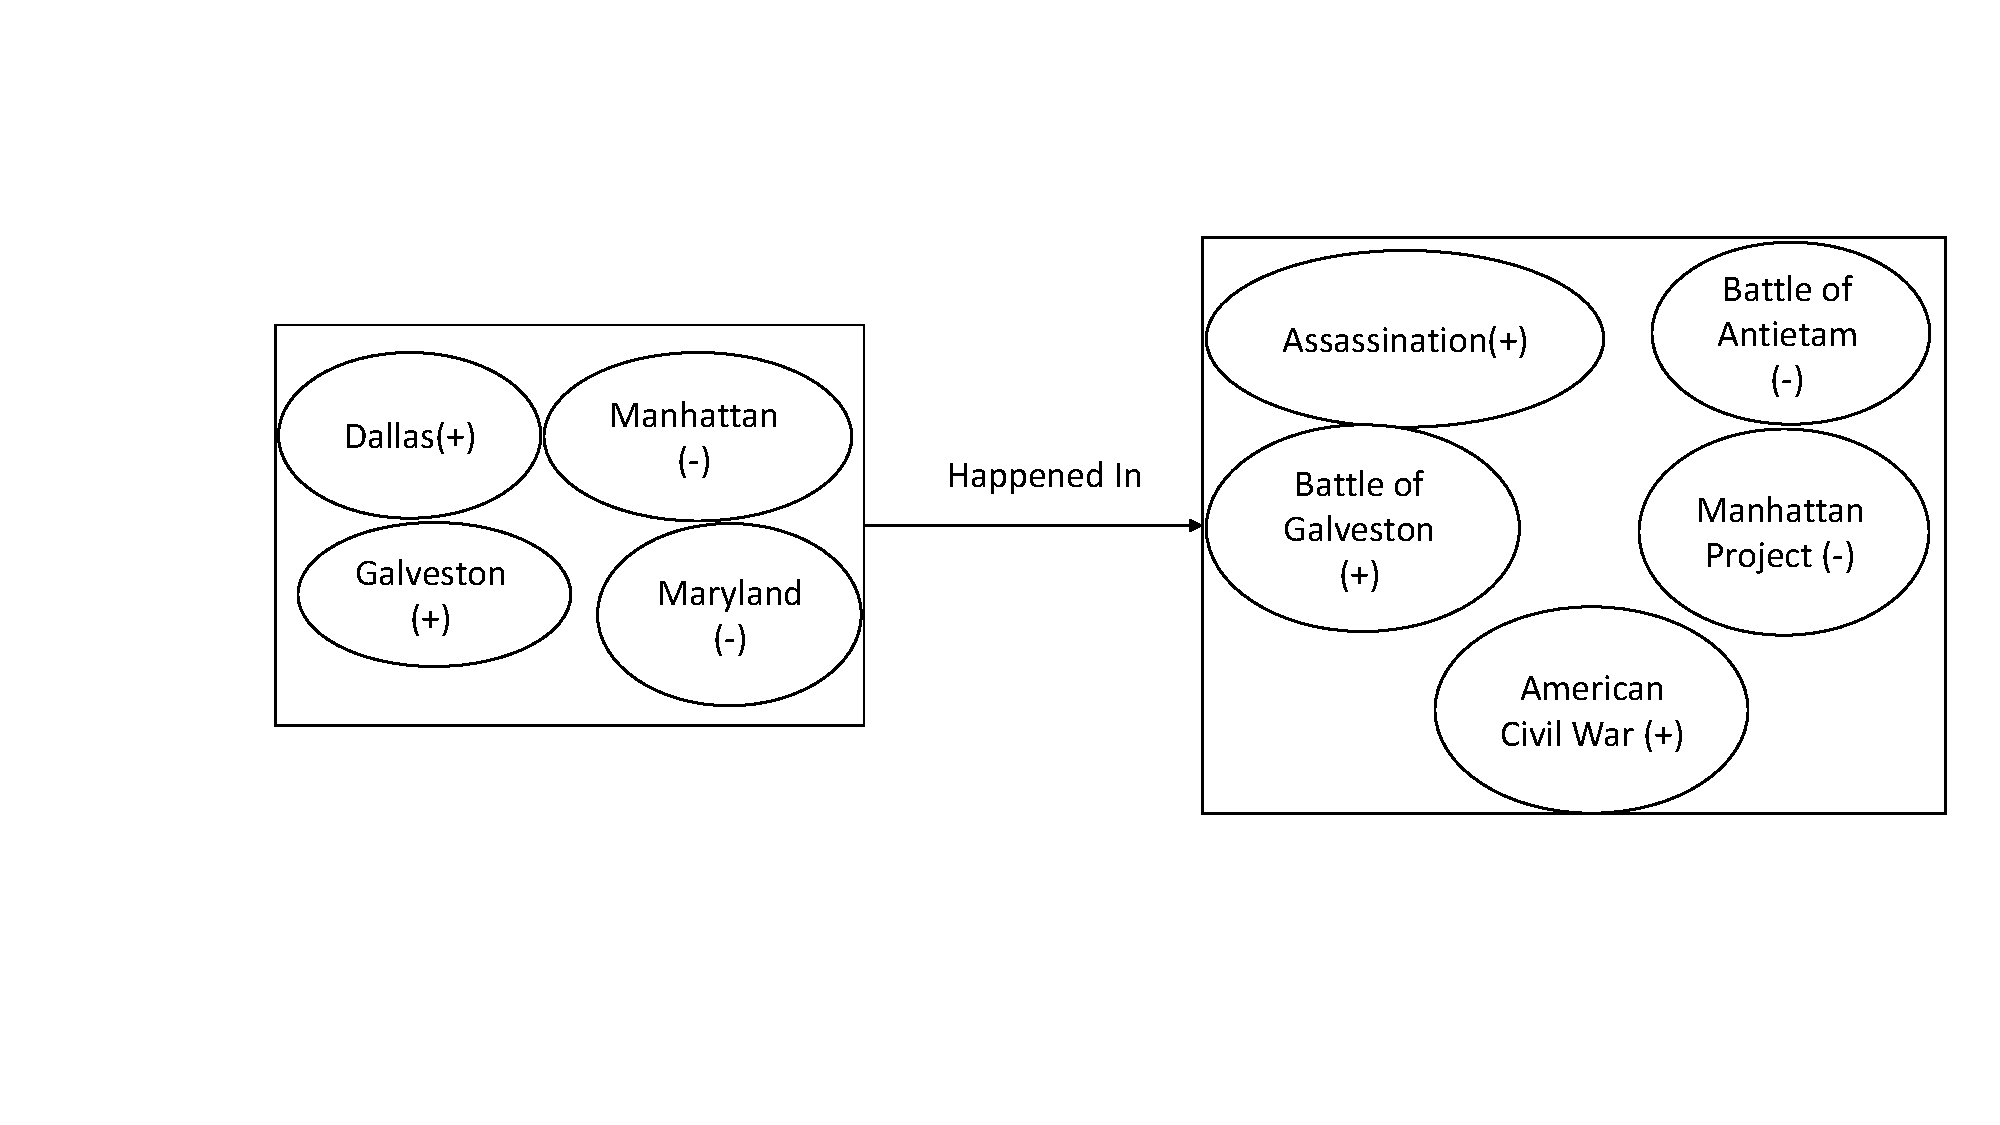
\includegraphics[width=0.7\linewidth]{figure_rec3_example_rec_new}
	\caption{Construction of a second level recursive learning problem based on the ``Happened in" relation. Feature values are treated as objects and labeled according to the labels of the problem on locations.}
	\label{fig:figure_rec3_example_rec}
\end{figure}

\begin{figure}[!h]
	\centering
	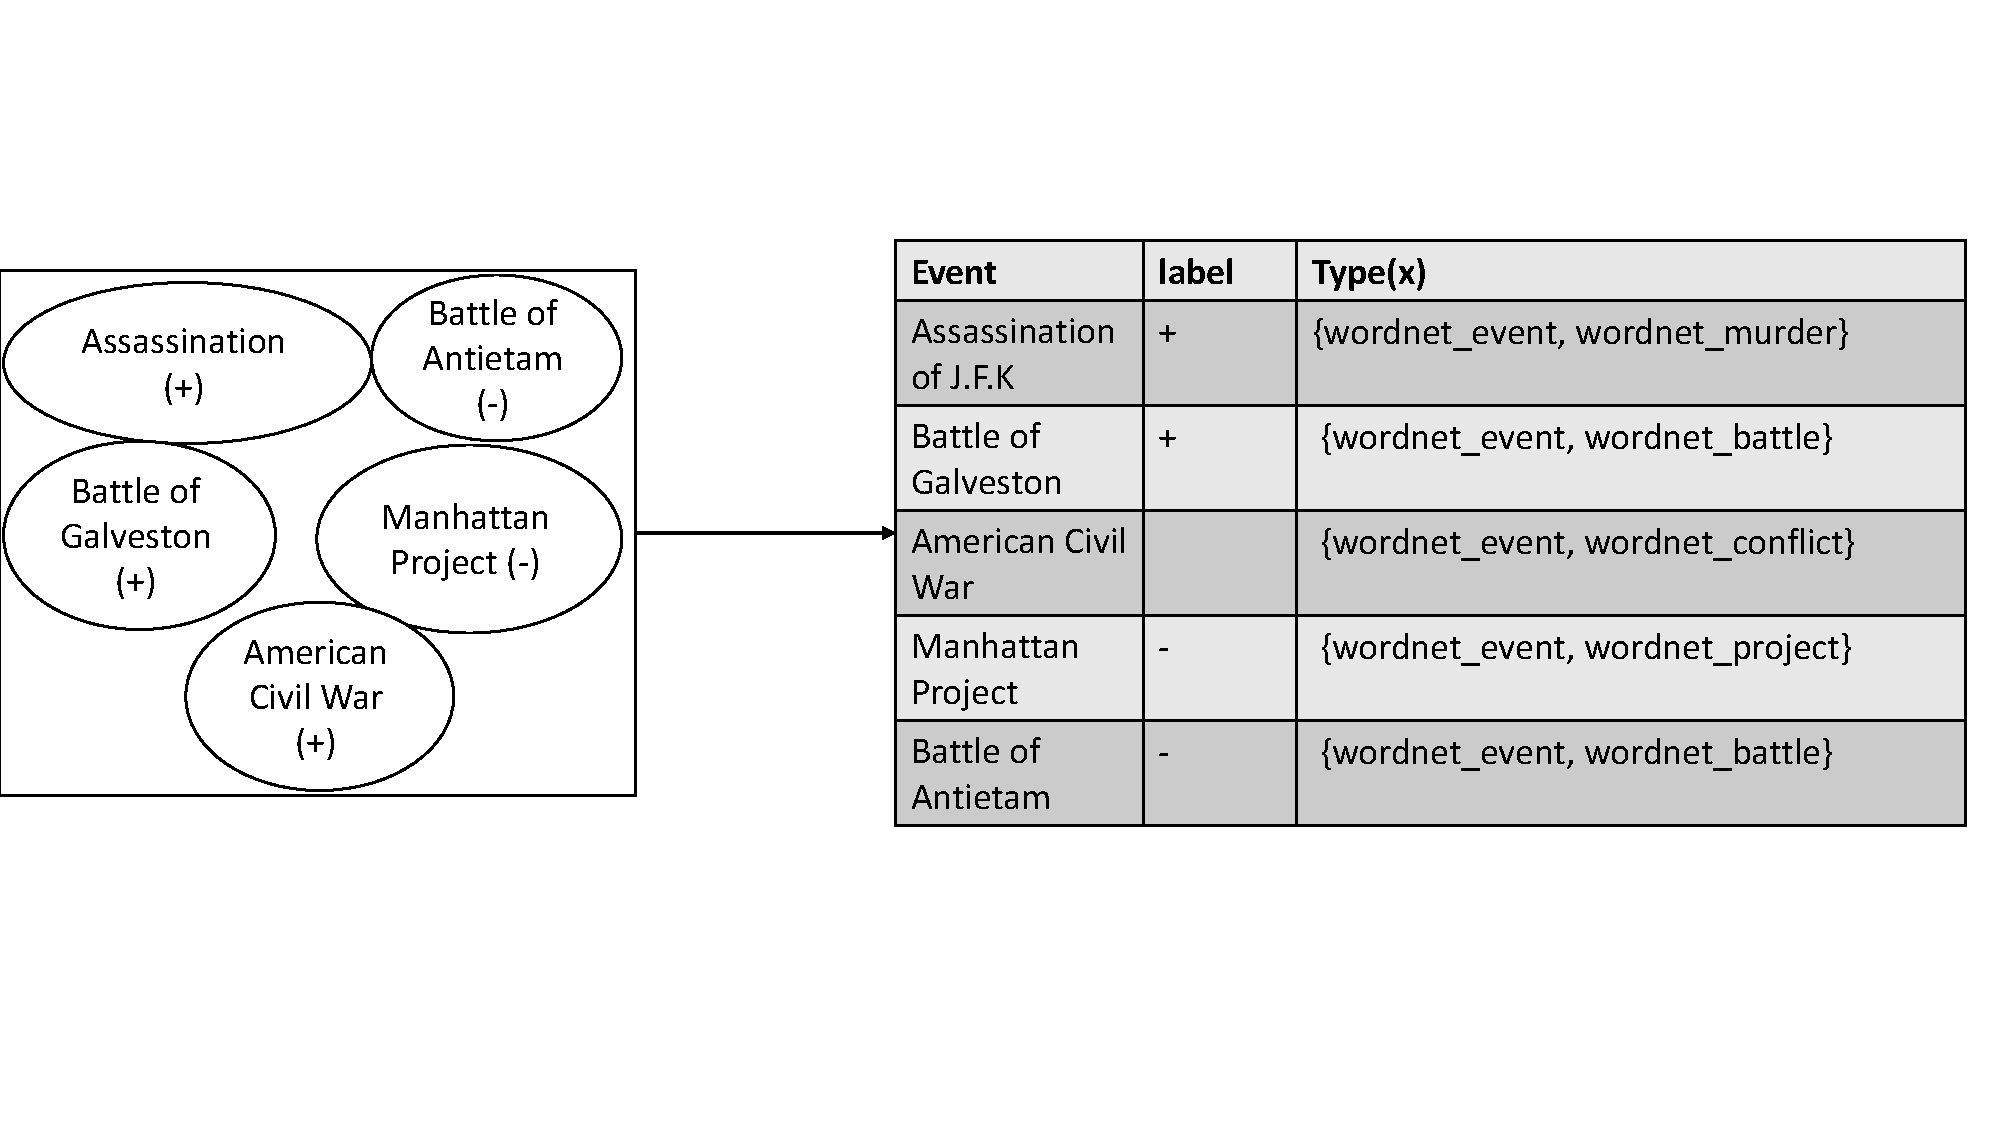
\includegraphics[width=\linewidth]{figure_rec3_problem_rec_new}
	\caption{Construction of a recursive learning problem based on the ``Happened in" relation. Once the example set has been created, applicable relations are used to create a feature set for the newly constructed induction problem.}
	\label{fig:figure_rec3_problem_rec}
\end{figure}

\begin{figure}[!h]
	\centering
	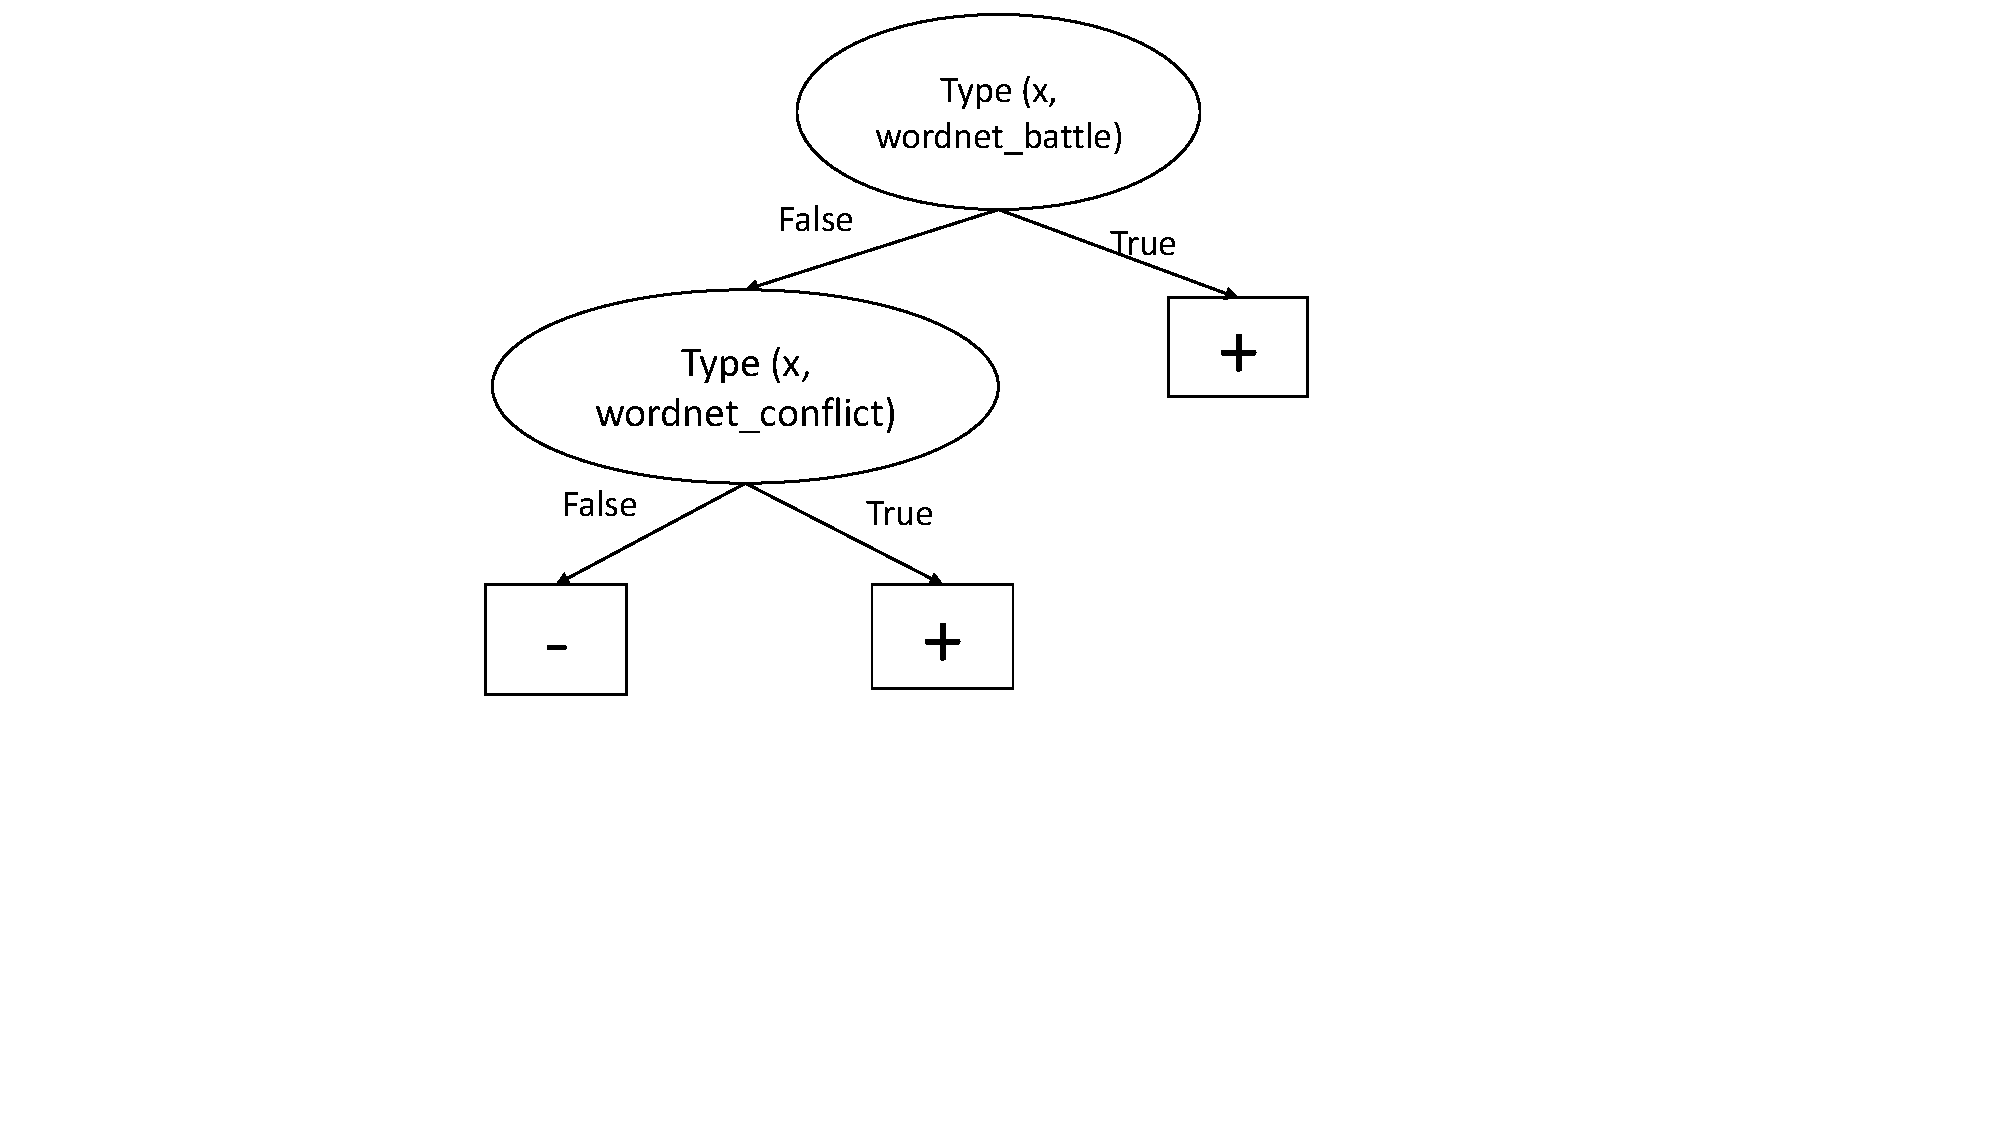
\includegraphics[width=0.4\linewidth]{figure_rec3_feature_rec_new}
	\caption{Recursive feature constructed by \emph{FEAGURE} for entities in the ``happened in" relation. This feature operates on events, and can be used in a classifier on locations.}
	\label{fig:figure_rec3_feature}
\end{figure}

Once we have generated this classifier on events, we can use it as a binary feature. \emph{FEAGURE} uses this new feature to expand the constructed induction problem on locations, shown in Figure \ref{fig:figure_rec3_problem}.
This feature is applied to a location through a majority vote over events that happened in that location. The result is a feature for locations representing the concept ``were most notable events in this location battles/conflicts?"
Finally, a decision tree learner is used on the expanded feature set to learn a classifier on locations to be used as a feature for our original learning problem. The new classifier for locations is shown in Figure \ref{fig:figure_rec3_feature_full}. It can be described as ``is this location located in Texas, or the site of battles or conflicts?".
Texts mentioning locations in and around Texas are more likely to link to locations that correspond to the output of this classifier.
We note that this feature was generated by \emph{FEAGURE}, and was later used by our external induction algorithm due to its high information gain. 

\begin{figure}[!h]
	\centering
	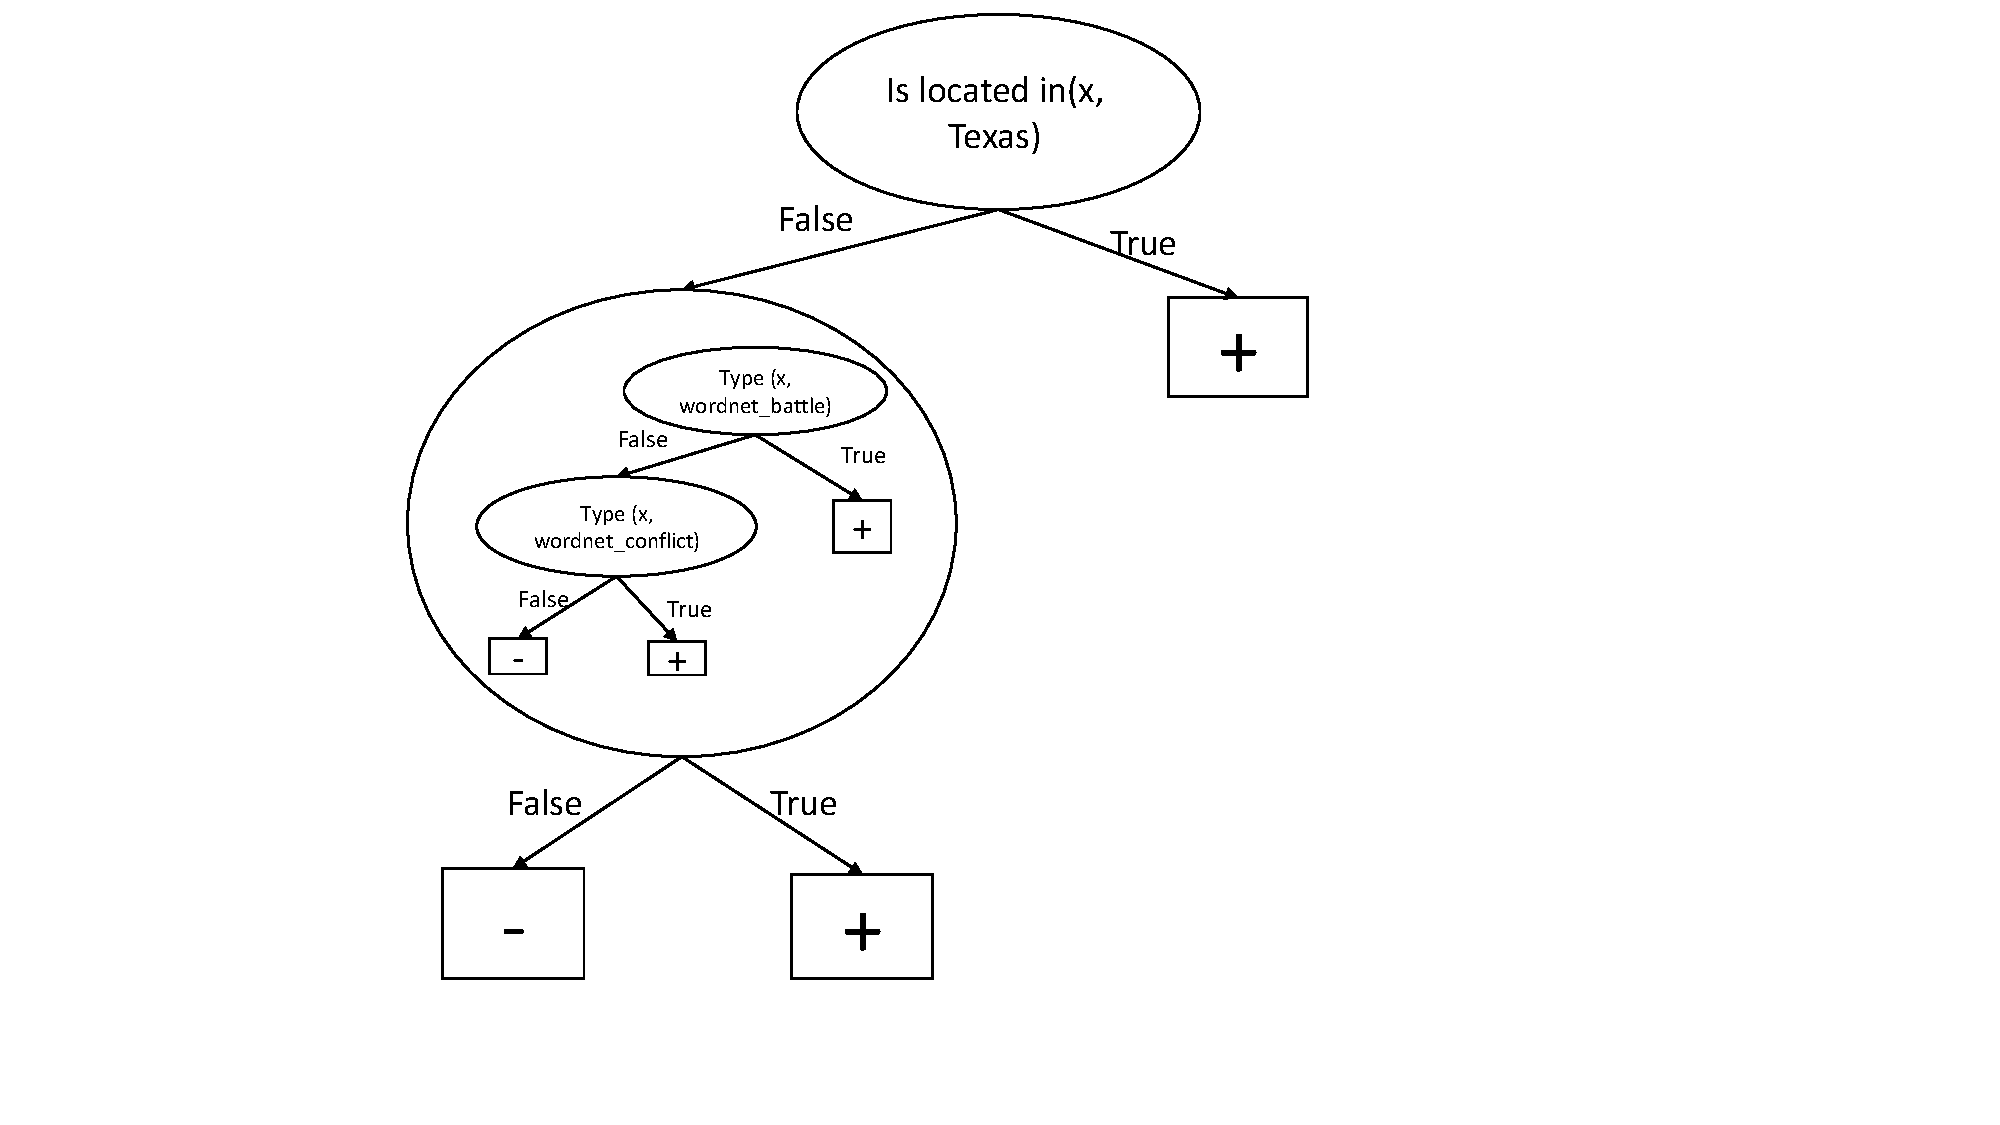
\includegraphics[width=0.6\linewidth]{figure_rec3_feature_new}
	\caption{Final generated feature constructed by \emph{FEAGURE} for entities in the ``located in" relation. The feature in the left branch is the recursive feature constructed by applying \emph{FEAGURE} to the new learning problem.}
	\label{fig:figure_rec3_feature_full}
\end{figure}

To conclude, we see that in general, good features created by \emph{FEAGURE} are those that are sufficiently broad in scope to group together a sizeable subset of similar entities. To this end, hypernyms can be very useful, as they group together entities in a taxonomy. 

\section{Related Work}

Many feature generation methodologies have been developed to search for new features that better represent the target concepts. There are three major approaches for feature generation: tailored methods, combinational techniques, and algorithms utilizing external knowledge.

Tailored approaches \cite{sutton1991learning,hirsh1994bootstrapping} are designed for specific problem domains and rely on domain-specific techniques. %for feature construction. 
One such example is the bootstrapping algorithm \cite{hirsh1994bootstrapping}, designed for the domain of molecular biology. The algorithm represents features as nucleotide sequences whose structure is determined by existing background knowledge. The algorithm uses an initial set of feature sequences, produced by human experts, and uses a domain-specific set of operators to change them into new sequence features. 
Such special-purpose algorithms  may be effectively tailored for a given domain, but have proven difficult to generalize to other domains and problems.

Combinational feature generation techniques are domain-independent methods for constructing more descriptive features by combining existing features in various ways. The LDMT algorithm \cite{utgo1991linear}, for example, performs feature construction in the course of building a decision-tree classifier. At each created tree node, the algorithm constructs a hyperplane feature through linear combinations of existing features in a way likely to produce concise, relevant hyperplanes. The LFC algorithm \cite{ragavan1993complex} combines binary features through the use of logical operators such as $\land ,\lnot$.
The FICUS algorithm \cite{markovitch2002feature} allows the use of any combinational feature generation technique, based on a given set of constructor functions. Recent work by \shortciteA{katz2016explorekit} uses a similar approach.

\emph{Deep Learning} \shortcite{rumelhart1986learning,lecun1998gradient} is another major class of combinational feature generation approaches. Here, the activation functions of the nodes can be viewed as feature schemes, which are instantiated during the learning process by changing the weights.

One limitation of combinational approaches is that they merely combine existing features to make the representation more suitable for the 
learning algorithm. 
Our \emph{FEAGURE} algorithm belongs to a third class of approaches that inject additional knowledge into the existing problem through the feature generation process.

Propositionalization approaches \shortcite{kramer2000bottom,cheng2011automatedfull} rely on relational data to serve as external knowledge. They use a combination of operators to create first-order logic predicates connecting existing data and relational knowledge. 
\citeA{cheng2011automatedfull} devised a generic propositionalization framework  using linked data via relation-based queries. 

FeGeLOD \cite{paulheim2012unsupervisedfull} also uses linked data to automatically enrich existing data. 
FeGeLOD uses feature values as entities and adds related knowledge from a relational knowledge base as new features to the existing examples. By doing so, FeGeLOD extends the feature set.

While these unsupervised approaches allow us to utilize external knowledge, any attempt to construct deep connections and relationships within the knowledge base will result in an exponential increase in the number of generated features.
To avoid this issue, \emph{FEAGURE} and other supervised approaches use the presence of labeled examples to better generate deeper features.

%TODO
Most supervised methods can trace their source to \emph{Inductive Logic Programming (ILP)} \cite{muggleton1991inductive}, a supervised approach that induces a set of first-order logical formulae to separate the different categories of examples in the training set.
ILP methods start from single relation formulae and add additional relational constraints using the knowledge base, until formulae that separate the training set into positive and negative examples are found. To that end, these approaches make use of a \emph{refinement operator}. When applied on a relational formula, this operator creates a more specialized case of that formula. For example, given the logical formula $BornIn(X,Y)$, where $X$ is a person and $Y$ is a city, one possible refinement is the formula $BornIn(X,Y)\land CapitalOf(Y,Z)$, where $Z$ is a country. The result is a logical formula that considers a more specific case. Additionally, we can look at a refinement that restricts by a constant, turning $BornIn(X,Y)$ into, for example, $BornIn(X, \mbox{{United States}})$. This refinement process continues until a sufficient set of consistent formulae is found. 

\emph{Relational Learning} techniques attempt to approach the problem of expanding knowledge from a different angle. These techniques are designed to expand an existing relational database. One such technique is View Learning \shortcite{davis2005view}. View learning uses labeled data to generate new relational tables from the existing relational knowledge.
It begins by applying ILP on relational data to construct new, simple, relational tables. Then,  using a Bayesian network induction algorithm, it learns ways to combine these relations into a single, more complex table.
This approach bears similarity to our approach in that it can effectively utilize background knowledge to draw conclusions using the combination of labeled data and background knowledge. These constructed tables attempt to fit new knowledge to existing examples, whereas our approach re-frames the learning problem within a new context.

The \emph{dynamic feature generation} approach used by the SGLR algorithm \cite{popescul200716} can be seen as the supervised equivalent of propositionalization methods. Instead of creating first-order predicates a priori, feature generation is performed during the training phase, allowing for complex features to be considered by performing a best-first search on possible candidates.
This process allows SGLR to narrow the exponential size of the feature space to a manageable number of candidates.
While this supervised approach overcomes the exponential increase in features that unsupervised approaches suffer from, the space of generated features that it searches is significantly less expressive than that of our approach.
Through the use of a recursive induction algorithm, our approach automatically locates relationships and combinations that we would not otherwise consider when using other approaches.

Kernel-based knowledge injection techniques aim to make use of powerful machine learning algorithms such as SVM by decoupling the knowledge base from the induction algorithm. This is done through the use of a kernel function that acts as a similarity function between examples in the problem domain. \shortciteA{losch2012graph}, for example, devised an approach that attempts to learn graph kernels within the relational domain. This process creates strong kernel functions that look at the neighborhood of an entity in search of similarities between entities. This  approach fundamentally differs from our own. Kernel methods attempt to create a filter through which entity similarity can be measured. In our approach, we attempt to locate the target concept through the use of different domains. This distinction is especially relevant to classification tasks, where many possible domains can apply for each example, and similarity may be difficult to find when considering the entire example set.

Another known method of utilizing external knowledge is Explanation-based Learning \shortcite{mitchell1986explanation,dejong1986explanation}, which uses a knowledge base of logical assertions to locate a small set of logical conditions that capture the target concept through deduction on examples from that concept. This approach uses deduction, rather than induction, as its main tool, allowing a logical knowledge base to be leveraged effectively.
However, due to the difficulty in creating good knowledge bases of logical assertions, this approach has shown limited success.

\citeA{terziev2011feature} shows an interesting approach to supervised feature generation. He proposes a decision tree based approach, where in each node of the tree, feature expansion is done using a method similar to that of FeGeLOD, with an entropy-based criterion to decide whether further expansion is required. This technique bears several similarities to \emph{Deep-FEAGURE} (Algorithm \ref{code-tree-thing}). However, the feature expansion process is unsupervised, and the resulting feature must be a decision tree, restricting the generality of the approach.

Since we have focused on the problem of text classification, we also discuss a few text-based approaches for feature generation. 
Linguistic methods such as those described in a study by \shortciteA{moschitti2004complex} attempt to use part-of-speech and grammar information to generate more indicative features than the bag-of-words representation of texts.
Concept-based approaches are the most similar to our own. Two examples of such methods are Explicit Semantic Analysis (ESA) \cite{gabrilovich2009wikipediafull},  which generates explicit concepts from Wikipedia based on similarity scores, and Word2Vec \shortcite{mikolov2013distributed}, which generates latent concepts based on a large corpus. Both approaches provide us with a feature set of semantic concepts. These concepts can be used alongside our approach, allowing us to induce over them.

\section{Conclusions}
%finishing up and summary

When humans use inductive reasoning to draw conclusions from their experience, they use a vast amount of general and specific knowledge. 
This use of knowledge allows us to reach better, more general conclusions.
In this paper we introduced a novel methodology for enhancing existing learning algorithms with background knowledge represented by relational knowledge bases.
The algorithm works by generating complex features induced using this external knowledge. It constructs recursive learning problems based on existing features and the knowledge base. These newly constructed problems are given as input to an induction algorithm. The output of this process is a collection of classifiers that are then turned into features for the original induction problem.

An important strength of our approach is its generality. The features generated by \emph{FEAGURE} can be used by any induction algorithm, allowing us to inject external knowledge in a general, algorithm independent manner.
One potential limitation of our approach is that it requires features with meaningful values. Nonetheless, for a wide range of problems, feature values do have meaning. For these problems, we can apply one of several general and domain-specific knowledge bases, depending on the problem.

In recent years, we have seen an increase in the number of available knowledge bases. These knowledge bases include general knowledge bases such as Freebase, YAGO, Wikidata and the Google Knowledge Graph, and more domain-specific knowledge bases,  from the British Geographical Survey (BGS) linked dataset, containing roughly one million geological facts regarding various geographical formations, through biological databases such as Proteopedia, composed of thousands of pages regarding biological proteins and molecules, to entertainment-focused databases such as IMDB, containing millions of facts on movies, TV series and known figures in the entertainment industry. 
With the recent surge in well-formed relational knowledge bases,
and the increasing prevalence of strong learning algorithms for a wide variety of tasks,
we believe our approach can take the performance of existing machine learning techniques to the next level.

\clearpage
\vskip 0.2in
\bibliographystyle{theapa}
\bibliography{document}

\end{document}

